\documentclass[supercite]{HustGraduPaper}
%进行个人信息设置
\title{双通道数字示波器} %论文题目
\author{裴熙隆} %作者姓名
\date{\today} %日期,默认当日
\school{人工智能与自动化学院} %院系名称
\classnum{自动化1705班} %专业班级
\stunum {U201714286} %学号
\instructor{王贞炎} %指导教师姓名

%添加自己要用的其他宏包
\usepackage{xltxtra}
\usepackage{bm}
\usepackage{array}
\usepackage{multirow}
\begin{document}
	%生成标题页 \maketitle[可选参数]
	%可选参数:
	%logo color=green/black 华中科技大学字样的颜色,绿色或者黑色,默认绿色
	%line length=12em 填写信息处横线的长度,默认12em
	%line font=huawenzhongsong 填写信息的字体,默认huawenzhongsong
	\maketitle
	
	%生成声明与授权书页 \statement[可选参数]
	%可选参数:
	%confidentiality=yes/no/true/false/empty 是否保密,yes/true为保密;no/false为不保密,empty为不填,默认为empty
	%year=5 保密年数,默认为空
%	\statement
	
	\clearpage %结束上一页
	\pagenumbering{Roman} %摘要页码为大写罗马数字
	
	%填写中文摘要内容和关键字
	\begin{cnabstract}{FPGA;电子测量;数字示波器}
		
		本双通道数字示波器以FPGA为核心,实现了双通道波形的采集与显示。通过高速ADC实时采样以获得较高的测量带宽,被测周期信号的频率范围为10Hz\textasciitilde10MHz。同时系统还具有参数测量、光标测量、档位切换、储存与调出波形等功能。本系统人机交互友好,刷屏帧率高,功能全面,性能指标优良,很好地完成了课程设计任务。		
		
		
	\end{cnabstract}

	%填写英文摘要内容和关键字
%	\begin{enabstract}{Key1; Key2; Key3}
%		Please Use English Semicolon and a Space "; " to Separate  Keys! 
%		
%		This is abstract. This is abstract. This is abstract. This is abstract. This is abstract. This is abstract. This is abstract. This is abstract. This is abstract. This is abstract. This is abstract. This is abstract. 
%		
%		This is abstract. This is abstract. This is abstract. This is abstract. This is abstract. This is abstract. This is abstract. This is abstract. This is abstract. This is abstract. This is abstract. This is abstract. 
%	\end{enabstract}
	
	%生成目录 \tableofcontents[可选参数]
	%可选参数:
	%pagenum=yes/no/true/false 目录是否显示页码,默认为false
	%toc in toc=yes/no/true/false 目录中是否有目录及其页码,默认为false
	%level=4 目录级数,默认是4,即显示到subsubsubsection
	%section indent=0em 目录第一级的缩进,默认是0em
	%subsection indent=1.5em 目录第二级的缩进,默认是1.5em
	%subsubsection indent=3.8em 目录第三级的缩进,默认是3.8em
	%subsubsubsection indent=7em 目录第四级的缩进,默认是7em
	%paragraph indent=11em 目录第五级的缩进,默认是11em
	%subparagraph indent=13em 目录第六级的缩进,默认13em
	%indent=normal/noindent/hustnoindent/sameforsubandsubsub 快速缩进设置,具体见文档
	%dot sep=4.5 目录点间距,默认4.5
	%section dot sep=4.5 目录第一级的点间距,默认是4.5
	%subsection dot sep=4.5 目录第二级的点间距,默认是4.5
	%subsubsection dot sep=4.5 目录第三级的点间距,默认是4.5
	%subsubsubsection dot sep=4.5 目录第四级的点间距,默认是4.5
	%paragraph dot sep=4.5 目录第五级的点间距,默认是4.5
	%subparagraph dot sep=4.6 目录第六级的点间距,默认是4.5
	%请注意在合适的位置放置\pagenumbering{numstyle}使用新的页码
	\tableofcontents
	
	\clearpage%结束上一页
	\pagenumbering{arabic} %正文页码为阿拉伯数字
	
	%正文内容从这里开始
	\section{系统方案设计}
	\subsection{系统方案描述}
	
	本设计实现的数字示波器,以 Xilinx的Zynq-7020系列FPGA为核心,利用搭载的ARM Cortex-A9处理器作为软件设计基础,实现了对被测信号的采样、显示、参数测量、光标测量、档位切换、触发功能切换、储存与调出等功能,通过高速ADC实时采样以获得较高的测量带宽。系统主要由信号调理、取样与保持、触发与控制逻辑四个部分组成,PL部分使用100MHz时钟驱动;可测量周期信号的频率范围为10Hz\textasciitilde10MHz,周期与电压测量误差均≤5\%;0.5V/div、0.2V/div、0.1V/div三个档位均能准确测量、显示波形;上升沿或下降沿触发方式、触发电平均可调节且验证无误;提供水平、垂直方向各两个测量光标,以及自动测量信号的频率、峰峰值、有效值、平均值、光标差值等参数,测量误差均≤1\%;当前显示的波形数据可以存储在板载的eMMC存储器中,随时调用。人机交互友好,刷屏帧率高,功能全面,所有指标均达到设计要求。
	
	\subsection{方案比较和选择}
	
	\subsubsection{采样逻辑设计方案}
	{\songti \bfseries 方案一:}FPGA逻辑根据当前选择的扫描档位来切换采样方式。
	
	{\songti \bfseries 方案二:}FPGA逻辑根据当前需要的采样率来切换采样方式。
	
	{\songti \bfseries 方案选择:}方案一,逻辑简单,易于实现,可以符合题目指标,但可扩展性不强;方案二,逻辑较复杂,但可扩展性强,可设置较多的采样率,从而设置更多的扫描档位。综合考虑,使用方案二。
	
	\subsubsection{信号调理方案}
	{\songti \bfseries 方案一:}使用一路放大器将各个档位的信号放大到合适值即可。
	
	{\songti \bfseries 方案二:}设置多档放大,分别设置不同的增益。
	
	{\songti \bfseries 方案选择:}方案一,部分档位输入信号过大,部分档位输入信号过小,不利于AD采集;方案二,电路复杂,但各个档位均能放大至AD输入最大范围,高效利用AD的动态范围,提高了系统的精度。综合考虑,使用方案二。
	
	\subsubsection{主控选择方案}
	{\songti \bfseries 方案一:}FPGA负责底层逻辑,用MCU做主控制器,它们之间通过SPI等串行通信接口通信。
	
	{\songti \bfseries 方案二:}FPGA负责底层逻辑,用软核处理器做主控制器。
	
	{\songti \bfseries 方案选择:}方案一,人机交互界面设计简单,但是FPGA与MCU之间数据通信不够可靠,通信速率成为了系统的瓶颈;方案二,软核与底层逻辑数据通信通过AXI总线,稳定可靠。虽然人机交互界面设计较为复杂,但是依然可以通过很多方式实现。综合考虑,使用方案二。
	
	\subsection{系统框图}
	系统框图如\autoref{fig:SystemDiagram}所示,两个通道的输入信号经过信号调理和换挡电路后由AD9288采集,通过并行数据总线输入FPGA,PL部分最终将数据通过DMA存储在DDR中,供PS部分进行读取。PS部分完成采样逻辑的控制和波形显示等人机交互部分,通过VDMA驱动显示器显示。
	\begin{generalfig}[htb]{系统框图}{fig:SystemDiagram}
		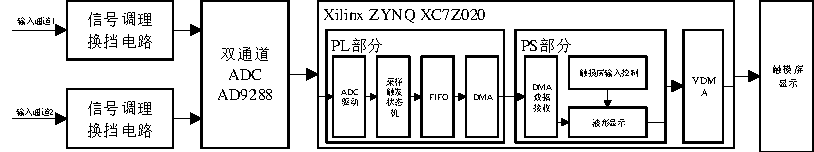
\includegraphics[width=\textwidth]{Figures/SystemDiagram.pdf}
	\end{generalfig}
	
	
	\section{相关原理和细节设计}
	\subsection{ADC选型及驱动}
	\subsubsection{ADC选型}
	题目要求最高水平速度为1us/div,共10个div,计算可得采样率要达到10MHz。垂直分辨率最高共100个点,因此需选用至少7位的ADC。将功能拓展为0.1us/div,并且双通道采样,则最高采样率为100MHz。综合考量,选用ADI公司的AD9288作为采样ADC,此ADC为双通道8位并行ADC,符合垂直分辨率的要求。
	
	\subsubsection{ADC驱动}
	ADC驱动负责产生AD9288的采样时钟、控制逻辑以及接收数据。
	
	AD9288为双通道8位并行ADC,最高可达100MHz的采样速率。示波器采用最高采样率,因此直接输出FPGA的系统时钟100MHz到ADC上作为采样时钟。由于输入端为时钟下降沿接收数据,所以输出时钟端口先经过反相器输入,输入信号则可用100MHz系统时钟上升沿触发接收数据,直接得到两个通道的采样数据,数据格式为偏移二进制,因此还要将MSB取反,得到补码形式的数据。
	
	\begin{generalfig}[htb]{AD9288采样时序图}{fig:AD9288TimingDiagram}
		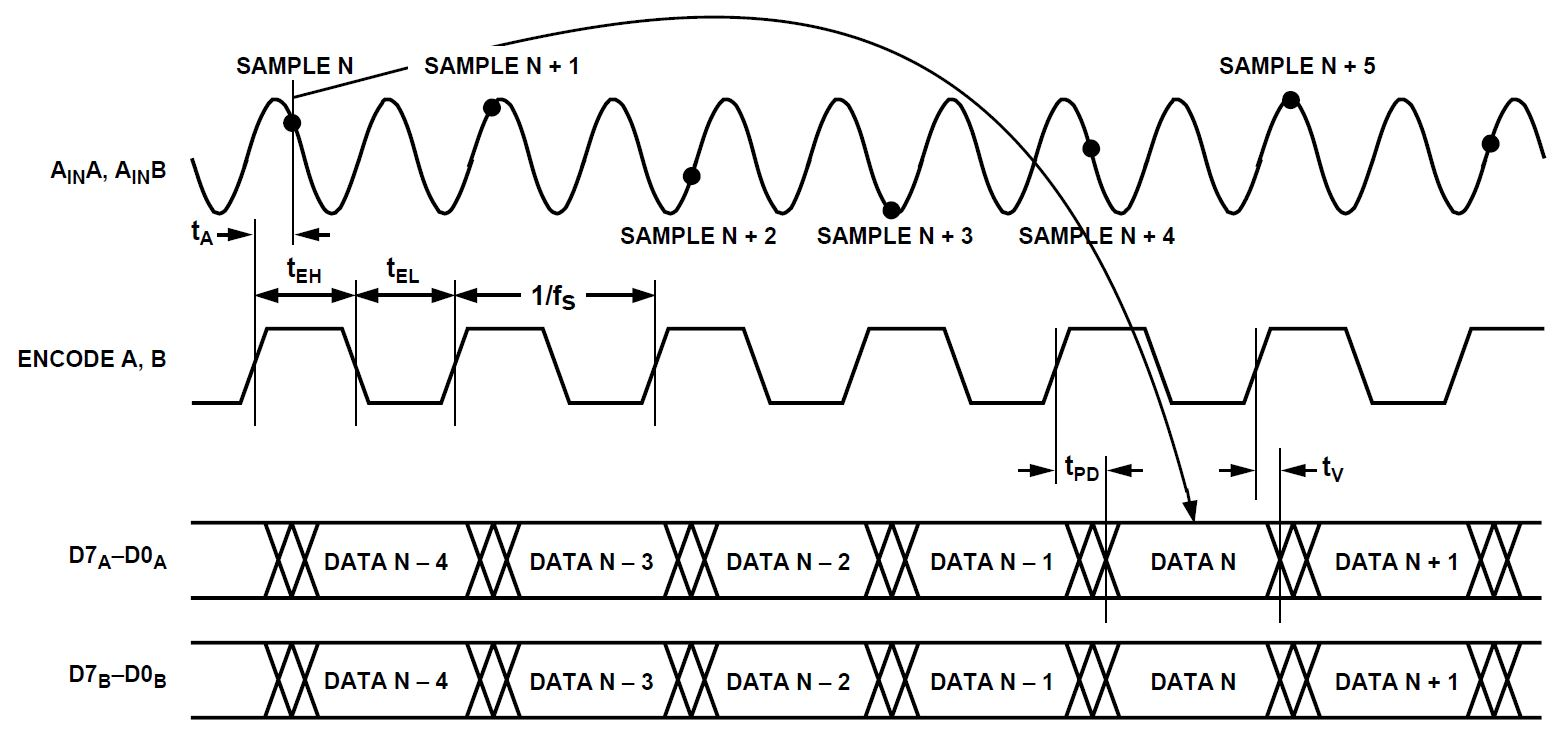
\includegraphics[width=\textwidth]{Figures/AD9288TimingDiagram.JPG}
	\end{generalfig}
	
	为避免输入的亚稳态效应,ADC并行数据进入FPGA后要先经过两级触发器,再送给下一级进行处理。AD9288的采样时序图如\autoref{fig:AD9288TimingDiagram}所示。
	
	\subsection{FPGA选型}
	FPGA采用Xilinx ZYNQ系列的XC7Z020作为主控,其框图如\autoref{fig:zynq-mp-core-dual}所示。该FPGA具有两个ARM Cortex-A9高性能应用级ARM处理器,PL部分有53.2k的LUT,106.4k的触发器,并且有1GB DDR3 SDRAM,4GB eMMC,满足题目使用要求。	
	
	\begin{generalfig}[htb]{Zynq-7000 SoC框图}{fig:zynq-mp-core-dual}
		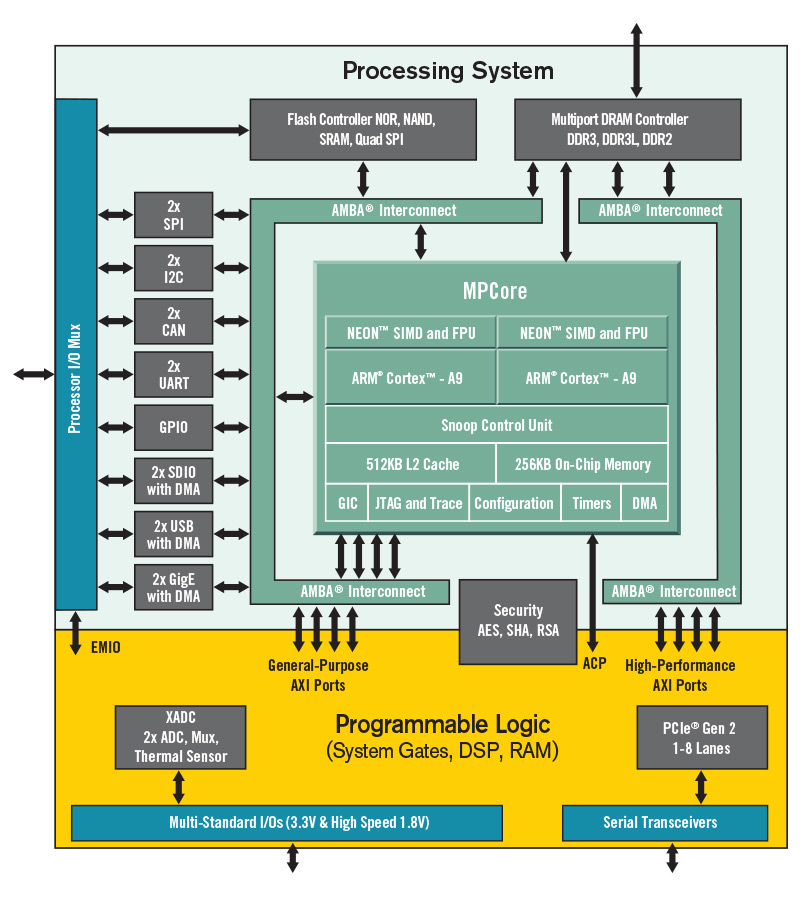
\includegraphics[width=10cm]{Figures/zynq-mp-core-dual.png}
	\end{generalfig}	
	
	\subsection{采样触发控制}
	示波器采样与触发系统负责对ADC的信号进行采样触发控制。
	
	触发系统同时还有水平档位切换功能,上升/下降沿触发,通道1/2触发控制,触发电平控制功能。采样系统一般持续接收数据。数据量超过设定的一帧数量,丢弃最早的数据,存入最新的数据,而在触发事件发生年后,在持续接收一定量的数据后停止。
	
	水平档位从小到大分别为0.1us/div,0.2us/div,0.5us/div,1us/div,2.5us/div,5us/div,10us/div,25us/div,50us/div,使用一个计数器产生使能信号控制速率,在100MHz的系统时钟下,计数器的模分别为0,1,4,9,24,49,99,249,499,将使能信号送到各个触发器块中,模的值通过处理器送来的寄存器值进行设置,从而实现在处理器中控制水平速率。
	
	上升/下降沿触发,触发通道切换通过处理器中送来的寄存器值进行修改,并带有10个单位的迟滞触发,以抵抗噪声带来的误触发。
	
	采样触发系统具有预触发功能,使用状态机对各个状态的切换进行控制。触发采样系统可以抽象出以下六种状态:
	
	(1)	空闲状态(IDLE):不采集。
	
	(2)	触发前采集状态(PRE):确保能采满用户设定的需要在触发事件到来前保留的数据量,在此状态下还需要对采集的数据计数,以便达到数量转换状态。
	
	(3)	等待触发状态(WAIT):等待触发事件的到来,同时也在采集数据,在此状态下也需要对已采集的数据计数,以便达到超时时间时转换状态。
	
	(4)	触发状态:满足用户设定的触发条件,开始触发后采样。
	
	(5)	超时状态:等待出发状态经历0.5s,强制采集一帧数据。
	
	(6)	后采样状态:满足触发条件或者已经超时,将数据采集满后结束采集。
	
	采样触发系统的状态转移如\autoref{fig:StateDiagram}所示。
	\begin{generalfig}[htb]{状态转移图}{fig:StateDiagram}
		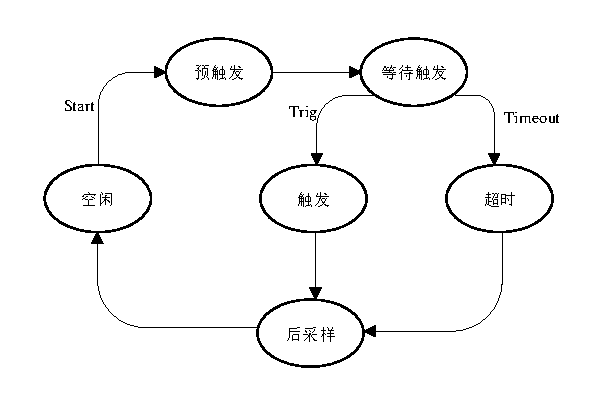
\includegraphics[width=10cm]{Figures/StateDiagram.pdf}
	\end{generalfig}		
	
	送给FIFO的数据共32位,其数据格式为:
	
	[7:0]:通道1数据;
	
	[15:8]:通道2数据;
	
	[16]:触发点处为1,其他为0;
	
	[17]:是否属于超时采样,是的话为1,否则为0;
	
	[31:18]:保留。
	
	\subsection{等精度频率测量}
	频率测量功能为了保证精确以及高性能,采用PL部分使用等精度频率计的技术进行测量。
	\begin{generalfig}[htb]{等精度频率测量原理}{fig:MeasuringPrinciple}
		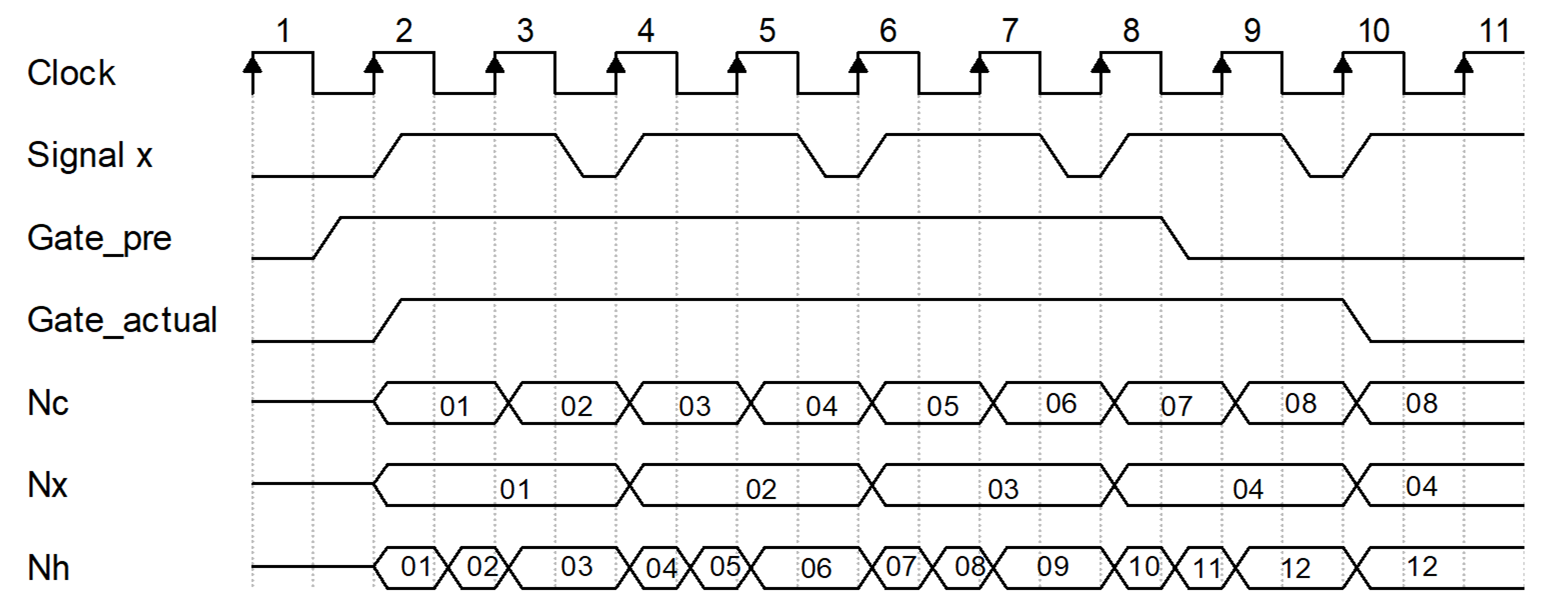
\includegraphics[width=10cm]{Figures/MeasuringPrinciple.png}
	\end{generalfig}

	如\autoref{fig:MeasuringPrinciple}所示,$ f_x $为待测信号频率,$ f_c $为标准时钟频率。两个计数器在同一闸门时间T内分别对待测信号、标准时钟进行计数,计数值为$ N_x $ 、$ N_c $。由于$ \frac{N_x}{f_x} = \frac{N_c}{f_c} = T $,则被测频率 $ f_x=\frac{N_x}{N_c} \cdot f_c $。
	
	利用D触发器使计数闸门信号与被测信号同步,开门时间T等于被测信号周期的整数倍,故$ N_x $无量化误差。则测频误差:
	\begin{equation}
	\frac{\Delta f_{x}}{f_{x}}=\pm\left(\frac{T_c}{T}+\left|\frac{\Delta f_{c}}{f_{c}}\right|+\frac{0.32}{k} \times 10^{-\frac{R}{20}}\right)
	\end{equation}
	式中$T_c$为$ N_c $计数器在同步门T期间的±1量化误差,$ \frac{\Delta f_{c}}{f_{c}} $为时钟$ f_c $的不确定度,$ R $为待测信号的信噪比,$ k $为多周期倍率。
	
	主要误差由$ T_c $引起,故$ \frac{\Delta f_{x}}{f_{x}}=\pm \frac{T_c}{T} $。时钟频率200MHz时,则$ T_c=50\mathrm{ns}  $,闸门选为0.2s,则$ N_c $计数误差$ \frac{T_c}{T} $为$ 5\times 10^{-9}  $。实测可测得的频率范围为DC\textasciitilde20MHz,测量精度大于十万分之一。
	
	将测得的数据通过AXI Lite总线将寄存器数据送到处理器中进行频率计算并显示。	
	
	\subsection{数据流接口设计}
	
	经过采样触发控制系统后,得到的数据要通过一个FIFO(First Input First Output)储存器,即先进先出的队列,送给DMA,从而与处理器进行数据同步。FIFO存储器是一个先入先出的双口缓冲器,即第一个进入其内的数据第一个被移出,其中一个是存储器的输入口,另一个口是存储器的输出口。使用Xilinx的IP的FIFO Generator实现,将接口格式设置为AXI Stream。
	
	由于示波器具有预触发功能,在数据采样后FIFO数据量大于采样长度时要将FIFO中的数据读出,同时要将FIFO的读接口接给DMA,即FIFO的Read端口连接两个部分,因此需要做逻辑控制,将FIFO的Read端口做切换,在示波器采样时将读端口送给示波器状态机做控制,在空闲时将读端口切换给DMA读取。其框图如\autoref{fig:AXIStream}所示。
	\begin{generalfig}[htb]{AXI Stream接口框图}{fig:AXIStream}
		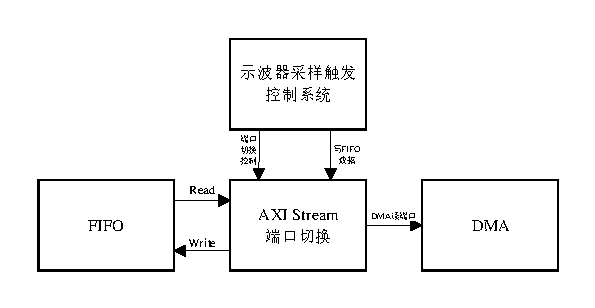
\includegraphics[width=\textwidth]{Figures/AXIStream.pdf}
	\end{generalfig}
	
	\subsection{DMA设计}
	为满足数据的高速读取操作,FIFO与处理器之间需使用DMA将FIFO的数据转移到内存DDR中供处理器使用。
	
	DMA(Direct Memory Access,直接内存存取)传输将数据从一个地址空间复制到另外一个地址空间。当CPU初始化这个传输动作,传输动作本身是由DMA控制器来实行和完成。典型的例子就是移动一个外部内存的区块到芯片内部更快的内存区。像是这样的操作并没有让处理器工作拖延,反而可以节省时间去处理其他的工作。
	
	使用Xilinx提供了IP来实现DMA,与FIFO通过AXI Stream接口读取数据,与处理器通过AXI SmartConnect连接到PS部分的AXI HP端口,将数据转移到内存中。FIFO与DMA接口的时序图如\autoref{fig:AXIStreamTimingDiagram}所示。
	
	\begin{generalfig}[htb]{FIFO与DMA的AXI Stream接口时序}{fig:AXIStreamTimingDiagram}
		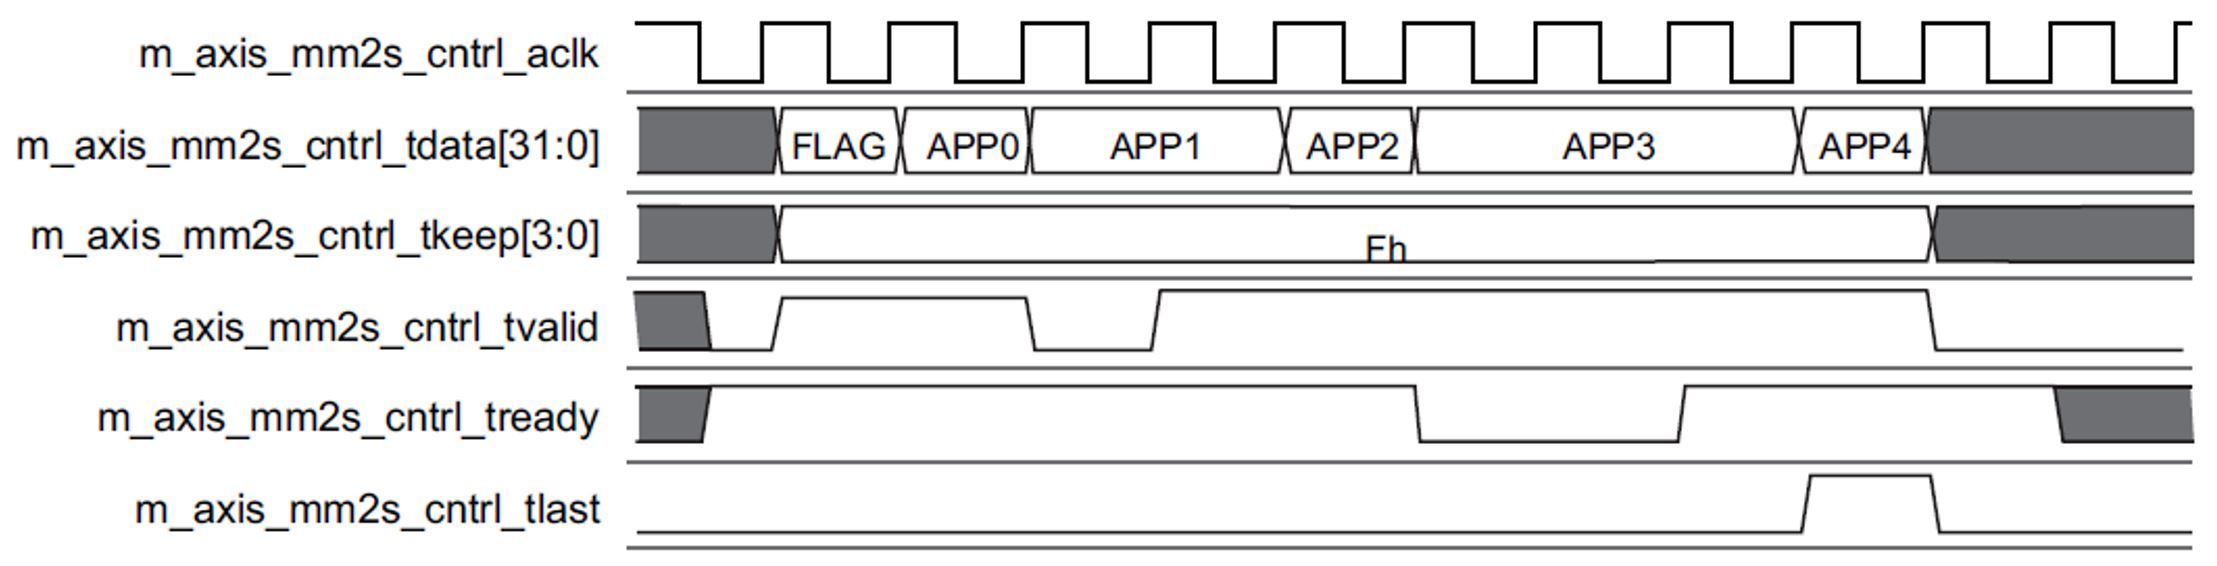
\includegraphics[width=\textwidth]{Figures/AXIStreamTimingDiagram.JPG}
	\end{generalfig}
	
	\subsection{液晶显示屏与人机交互}
	
	为了更好地实现人机交互,选用微雪电子7寸液晶显示屏进行显示,分辨率为1024×600,可以很好地显示当前采样得到的波形,且自带轮询触摸检测,检测到触摸后,由屏幕内部控制芯片在I2C接口上产生对应的信息,传送到FPGA板上,再由顶层触发中断,解析数据,得到触摸点坐标并进行相应的操作。\autoref{fig:LCDInfo}所示为显示屏的基本信息。
	
	\begin{generalfig}[htb]{LCD显示屏基本信息}{fig:LCDInfo}
		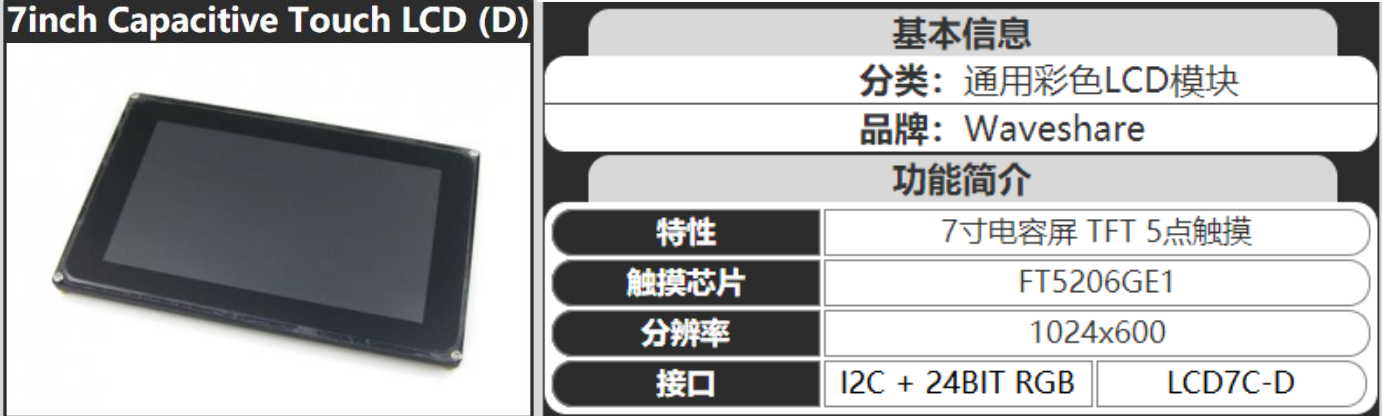
\includegraphics[width=\textwidth]{Figures/LCDInfo.PNG}
	\end{generalfig}
	
	触摸屏中断信号INT为低电平有效。当手指触摸电容屏时,INT信号会以固定频率(默认为 60Hz)脉冲信号的形式输出,当手指离开电容屏,INT信号重新恢复高电平,如\autoref{fig:LCDINTTiming}所示,本质上看就是一种IIC的传输方式,我们正是利用了这个信号,来控制触摸。
	
	\begin{generalfig}[htb]{触摸屏中断时序图}{fig:LCDINTTiming}
		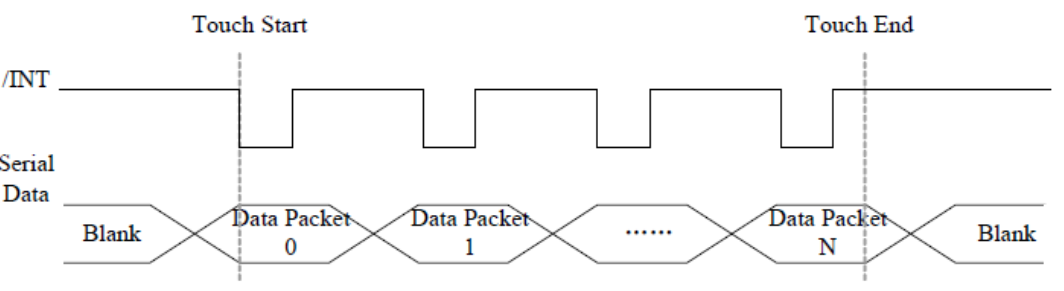
\includegraphics[width=10cm]{Figures/LCDINTTiming.png}
	\end{generalfig}
	
	得到触摸信号之后,根据I2C传来的串行寄存器数据来读取信息,查阅显示屏的数据手册,可以得到\autoref{fig:LCDRegTable}所示的寄存器表。
	
	\begin{generalfig}[htb]{LCD寄存器表}{fig:LCDRegTable}
		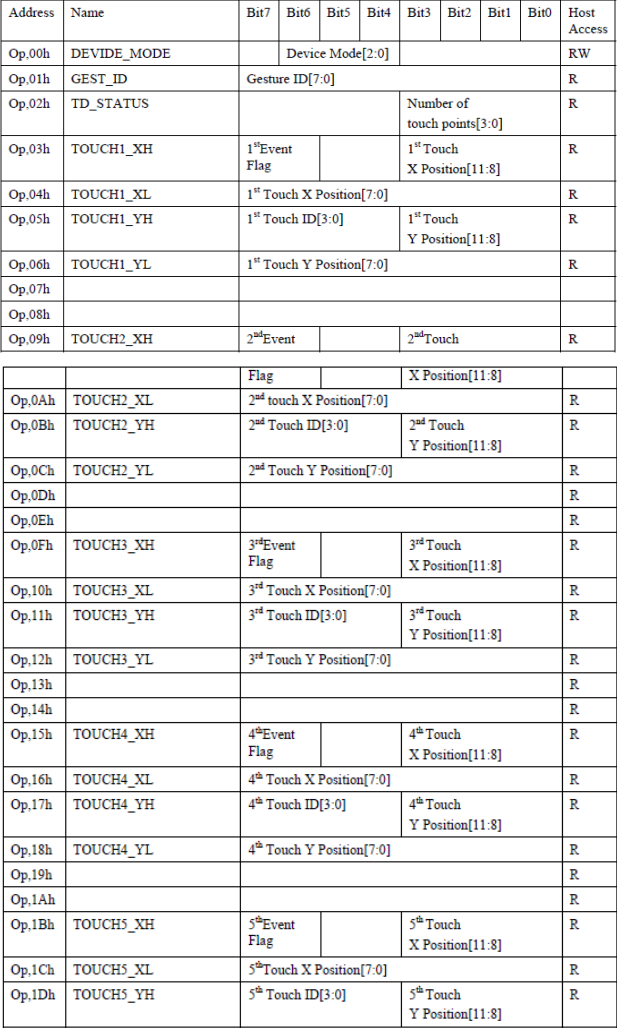
\includegraphics[width=8cm]{Figures/LCDRegTable.png}
	\end{generalfig}
	
	其中,TD\_STATUS寄存器记录了触摸点数,因此接收到中断标志之后,首先读取寄存器地址,再读取数据,整个接口时序符合I2C标准。
	
	\subsection{视频流直接存储器访问(Vedio DMA)}
	由于使用VDMA可以方便地实现双缓冲和多缓冲机制,所以本小节引入了帧缓存和缓冲机制的概念。另外,VDMA可以很好地契合Zynq内部架构,缩短开发周期。再加上VDMA本身能够高效地实现数据存取,所以在基于Zynq(也包括其他Xilinx FPGA)的图像、视频处理系统中,VDMA可谓是必不可少的。
	
	而VDMA涉及到缓存的概念。缓冲存储器(Frame Buffer):简称帧缓存或显存,它是屏幕所显示画面的一个直接映象,又称为位映射图(Bit Map)或光栅。帧缓存的每一存储单元对应屏幕上的一个像素,整个帧缓存对应一帧图像。在开发者看来,Frame Buffer 是一块显示缓存,往显示缓存中写入特定格式的数据就意味着向屏幕输出内容。所以说Frame Buffer就是一块画布,系统在画布上绘制好画面之后,就可以通知显示设备读取Frame Buffer进行显示了。
	
	在具体的项目实现中,对VDMA的调用经常采用双缓冲机制来加速显示以及提高帧率,双缓冲机制的原理图如\autoref{fig:DoubleBuffering}所示。
	
	\begin{generalfig}[htb]{双缓冲示意图}{fig:DoubleBuffering}
		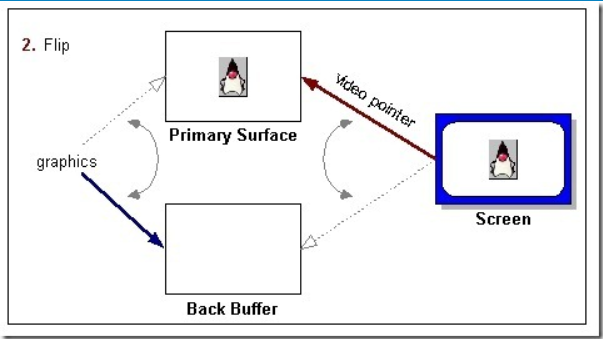
\includegraphics[width=10cm]{Figures/DoubleBuffering.png}
	\end{generalfig}
	
	
	最早解释多缓冲区如何工作的方式,是通过一个现实生活中的实例来解释的,这里花一些篇幅加以描述。
	
	{\songti \bfseries 单缓冲:}在一个阳光明媚的日子,你想将水池里的水打满,而又找不到水管的时候,就只能用手边的木桶来灌满水池。水桶满了之后,关掉水龙头,将水提到水池旁边,倒进去,然后走回到水龙头。重复上述工作,如此往复直到将水池灌满。这就类似单缓冲工作过程,当你想将木桶里的水倒出的时候,你必须关掉水龙头。
	
	{\songti \bfseries 双缓冲:}现在假设有人用两个木桶来做上面的工作。你会注满第一个木桶然后将第二个木桶换到水龙头下面,这样,在第二个水桶注满的时间内,你就可以将第一个木桶里面的水倒进水池里面,当你回来的时候,你只需要再将第一个木桶换下第二个注满水木桶,当第一个木桶开始注水的时候你就将第二个木桶里面的水倒进水池里面。重复这个过程直到水池被注满。
	
	很容易看得到用这种技术注满水池将会更快,同时也节省了很多等待木桶被注满的时间,而这段时间里你什么也做不了,而水龙头也就不用等待从木桶被注满到你回来的这段时间了。
	
	当你雇佣另外一个人来搬运一个被注满的木桶时,这就有点类似于三个缓冲区的工作原理。如果将搬运木桶的的时间很长,你可以用更多的木桶,雇佣更多的人,这样水龙头就会一直开着注满木桶了。
	
	在计算机图形学中,双缓冲是一种画图技术,使用这种技术可以使得画图没有(至少是减少)闪烁、撕裂等不良效果,并减少等待时间。双缓冲机制的原理大概是:所有画图操作将它们画图的结果保存在一块系统内存区域中,这块区域通常被称作“后缓冲区(Back Buffer)”,当所有的绘图操作结束之后,将整块区域复制到显示内存中,这个复制操作通常要跟显示器的光栈束同步,以避免撕裂。双缓冲机制必须要求有比单缓冲更多的显示内存和CPU消耗时间,因为“后缓冲区”需要显示内存,而复制操作和等待同步需要CPU时间。
	
	Xilinx 提供的VDMA IP核的几个重要信号,在这里列举。
	
	{\songti \bfseries Frame Buffers :}选择VDMA缓存几帧图像,这里默认是写通道和读通道都设置相同的缓存帧数,具体设置多少帧合适一般根据应用来定,比如读写带宽相同,想用DDR作为一个乒乓Buffer,那就可以设置成2帧,写第一个地址,读第二个地址,然后写第二个地址,读第一个地址。这里面设置几帧,就要在VDMA寄存器配置的时候设置几个帧起始地址。 
	
	{\songti \bfseries Memory Map Data Width:}代表数据到达AXI4总线上的位宽,比如这里设置成64,那就代表M\_AXI\_XX总线上的数据位宽是64bit,这时候如果Stream上的数据是32bit,那VDMA内部会有一个带宽转换模块,把数据拼成64bit。 
	
	{\songti \bfseries Burst Size :}AXI总线上突发传输的长度,一般设置为16。
	
	{\songti \bfseries Stream Data Width:}VDMA与PL逻辑部分通过AXI Stream协议交互数据,这里代表Stream数据位宽。
	
	{\songti \bfseries Line Buffer Depth:}VDMA内部会有一个行缓存FIFO,Stream数据会先写入FIFO,然后AXI总线逻辑会读出到总线上,这个深度就代表FIFO的深度。设置原则(个人理解):如果AXI总线数据带宽是Stream总线数据带宽的1.5倍以上,这个FIFO深度可以设置的小一点,如果AXI总线带宽小于1.5倍的Stream总线带宽,那FIFO的深度至少要是图像一个有效行的一半。 
	
	\subsection{时序控制器(Video Timing Controller)}
	使用VDMA来传送显示的数据,还需要有正确的时钟信号来控制VDMA从DDR内存里搬移数据,以及转化成RGB接口输出。这一工作是由时序控制器VTC来完成的,Xilinx官方有提供时序控制器的IP核,为节约开发时间,直接调用。
	
	所有视频系统都需要管理视频定时信号,该视频定时信号用于同步各种过程。视频定时控制器具有检测和生成这些定时信号的功能。\autoref{fig:ExampleVedioFrameAndTimingSignals}显示了包括定时信号的典型视频帧。
	\begin{generalfig}[htb]{视频帧和定时信号示例}{fig:ExampleVedioFrameAndTimingSignals}
		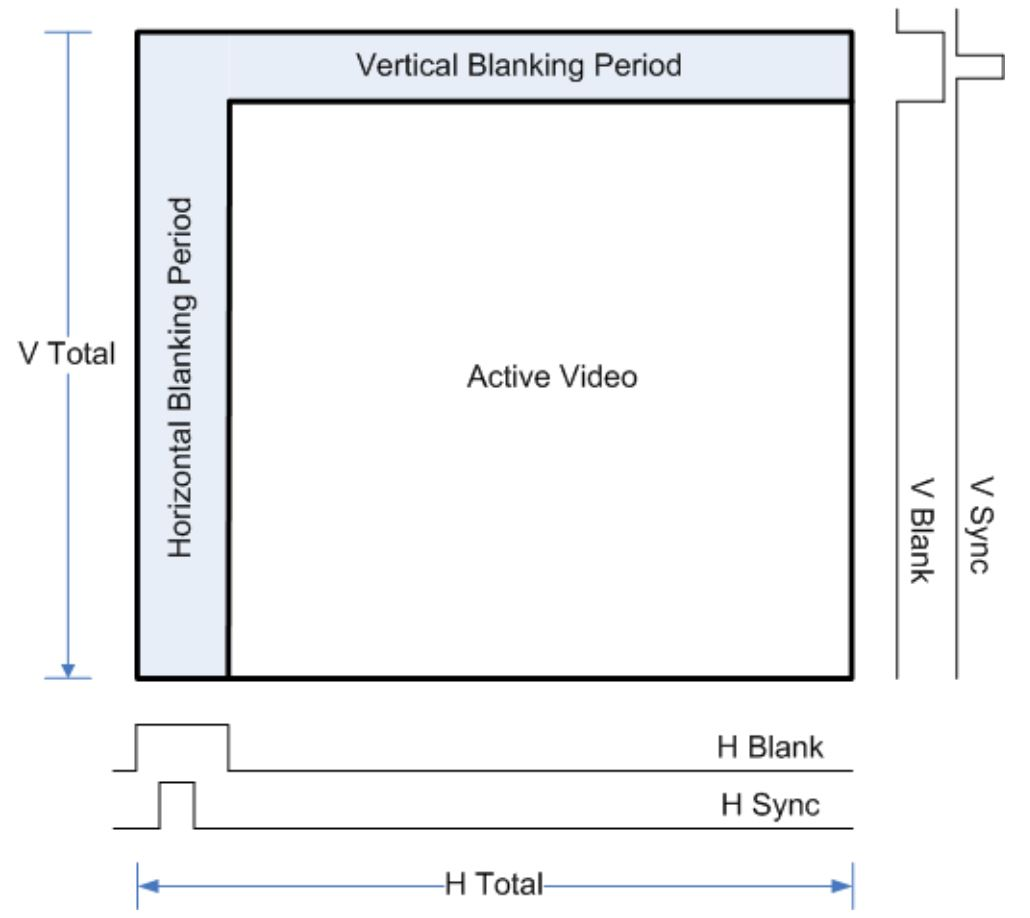
\includegraphics[width=10cm]{Figures/ExampleVedioFrameAndTimingSignals.JPG}
	\end{generalfig}

	\subsection{LCD背光控制}
	LCD显示屏需要用到背光控制,背光采用脉冲宽度调制进行控制。因此需要设计PWM模块生成脉冲宽度调制信号,输出给显示器。
	
	为了减小开发周期,我们采用Digilent公司的AXI PWM IP核来生成脉冲宽度调制信号。另外,此IP核可以在软件中随时配置PWM信号的参数(如频率、占空比等等),使用较为灵活。
	\subsection{波形数据存储}
	为了存储示波器的当前波形,我们比较了SD卡和eMMC两种存储方式,最终决定使用eMMC来存储波形数据,原因在于eMMC拥有较快的读写速度,且配置起来较为方便,减少开发周期和调试难度。
	
	嵌入式多媒体卡(Embedded Multimedia Card)是一种新的存储技术,由MMC协会所订立。该架构标准将MMC组件(闪存加控制器)放入一个小的球栅数组封装(BGA)中,是一种主要用于印刷电路板的嵌入式非易失性存储器系统。eMMC有100、153、169个触点之分,并都基于8位并行接口。eMMC与MMC的其他版本有明显的不同,因为eMMC不是用户可随意移动的卡,而是永久性的电路板附件。如果eMMC出现内存或其控制器的问题,则可能需要更换整个PCB(印刷电路板)来修复。
	
	几乎所有在2016年之前生产的手机和平板电脑都使用这种形式的主存储器,直到2016年UFS开始渐渐占领市场。JEDEC的最新的eMMC标准(JESD84-B51)是在2015年2月发布的5.1版本,该版本的eMMC速度可媲美SATA接口标准的固态硬盘(400 MB/s),\autoref{tab:eMMC}简述 了不同版本的eMMC的写入速度和读取速度。
	
	\begin{generaltab}{不同版本的eMMC的写入速度和读取速度}{tab:eMMC}
		\begin{tabularx}{10cm}{CCC}
			\toprule
			& 写入速度(MB/s) & 读取速度(MB/s)      \\
			\midrule
			eMMC 5.1 & 125      & 250      \\
			eMMC 5.0 & 90       & 250      \\
			eMMC 4.5 & 50       & 140      \\
			\bottomrule
		\end{tabularx}
	\end{generaltab}

	由此看来,可以说eMMC的读写速度远超SD卡,综上所述,选用eMMC读写方案。由于FPGA开发板已经具备板载的eMMC,只需要配置存储器接口即可使用,在PS配置中勾选SD卡接口,将其连接到eMMC,即可实现复用。

	\section{电路设计}
	\subsection{信号调理电路}
	信号调理电路主要由挡位切换电路以及抗混叠滤波电路组成。其中,挡位切换电路选用TI公司的精密运放OPA656搭建交流耦合电压跟随器,其后跟三路不同放大倍数的电阻分压电路,通道A、B、C分别对应放大1倍、0.5倍、0.2倍,电路图如\autoref{fig:SwitchCircuit}所示。
	
	\begin{generalfig}[htb]{挡位切换电路}{fig:SwitchCircuit}
		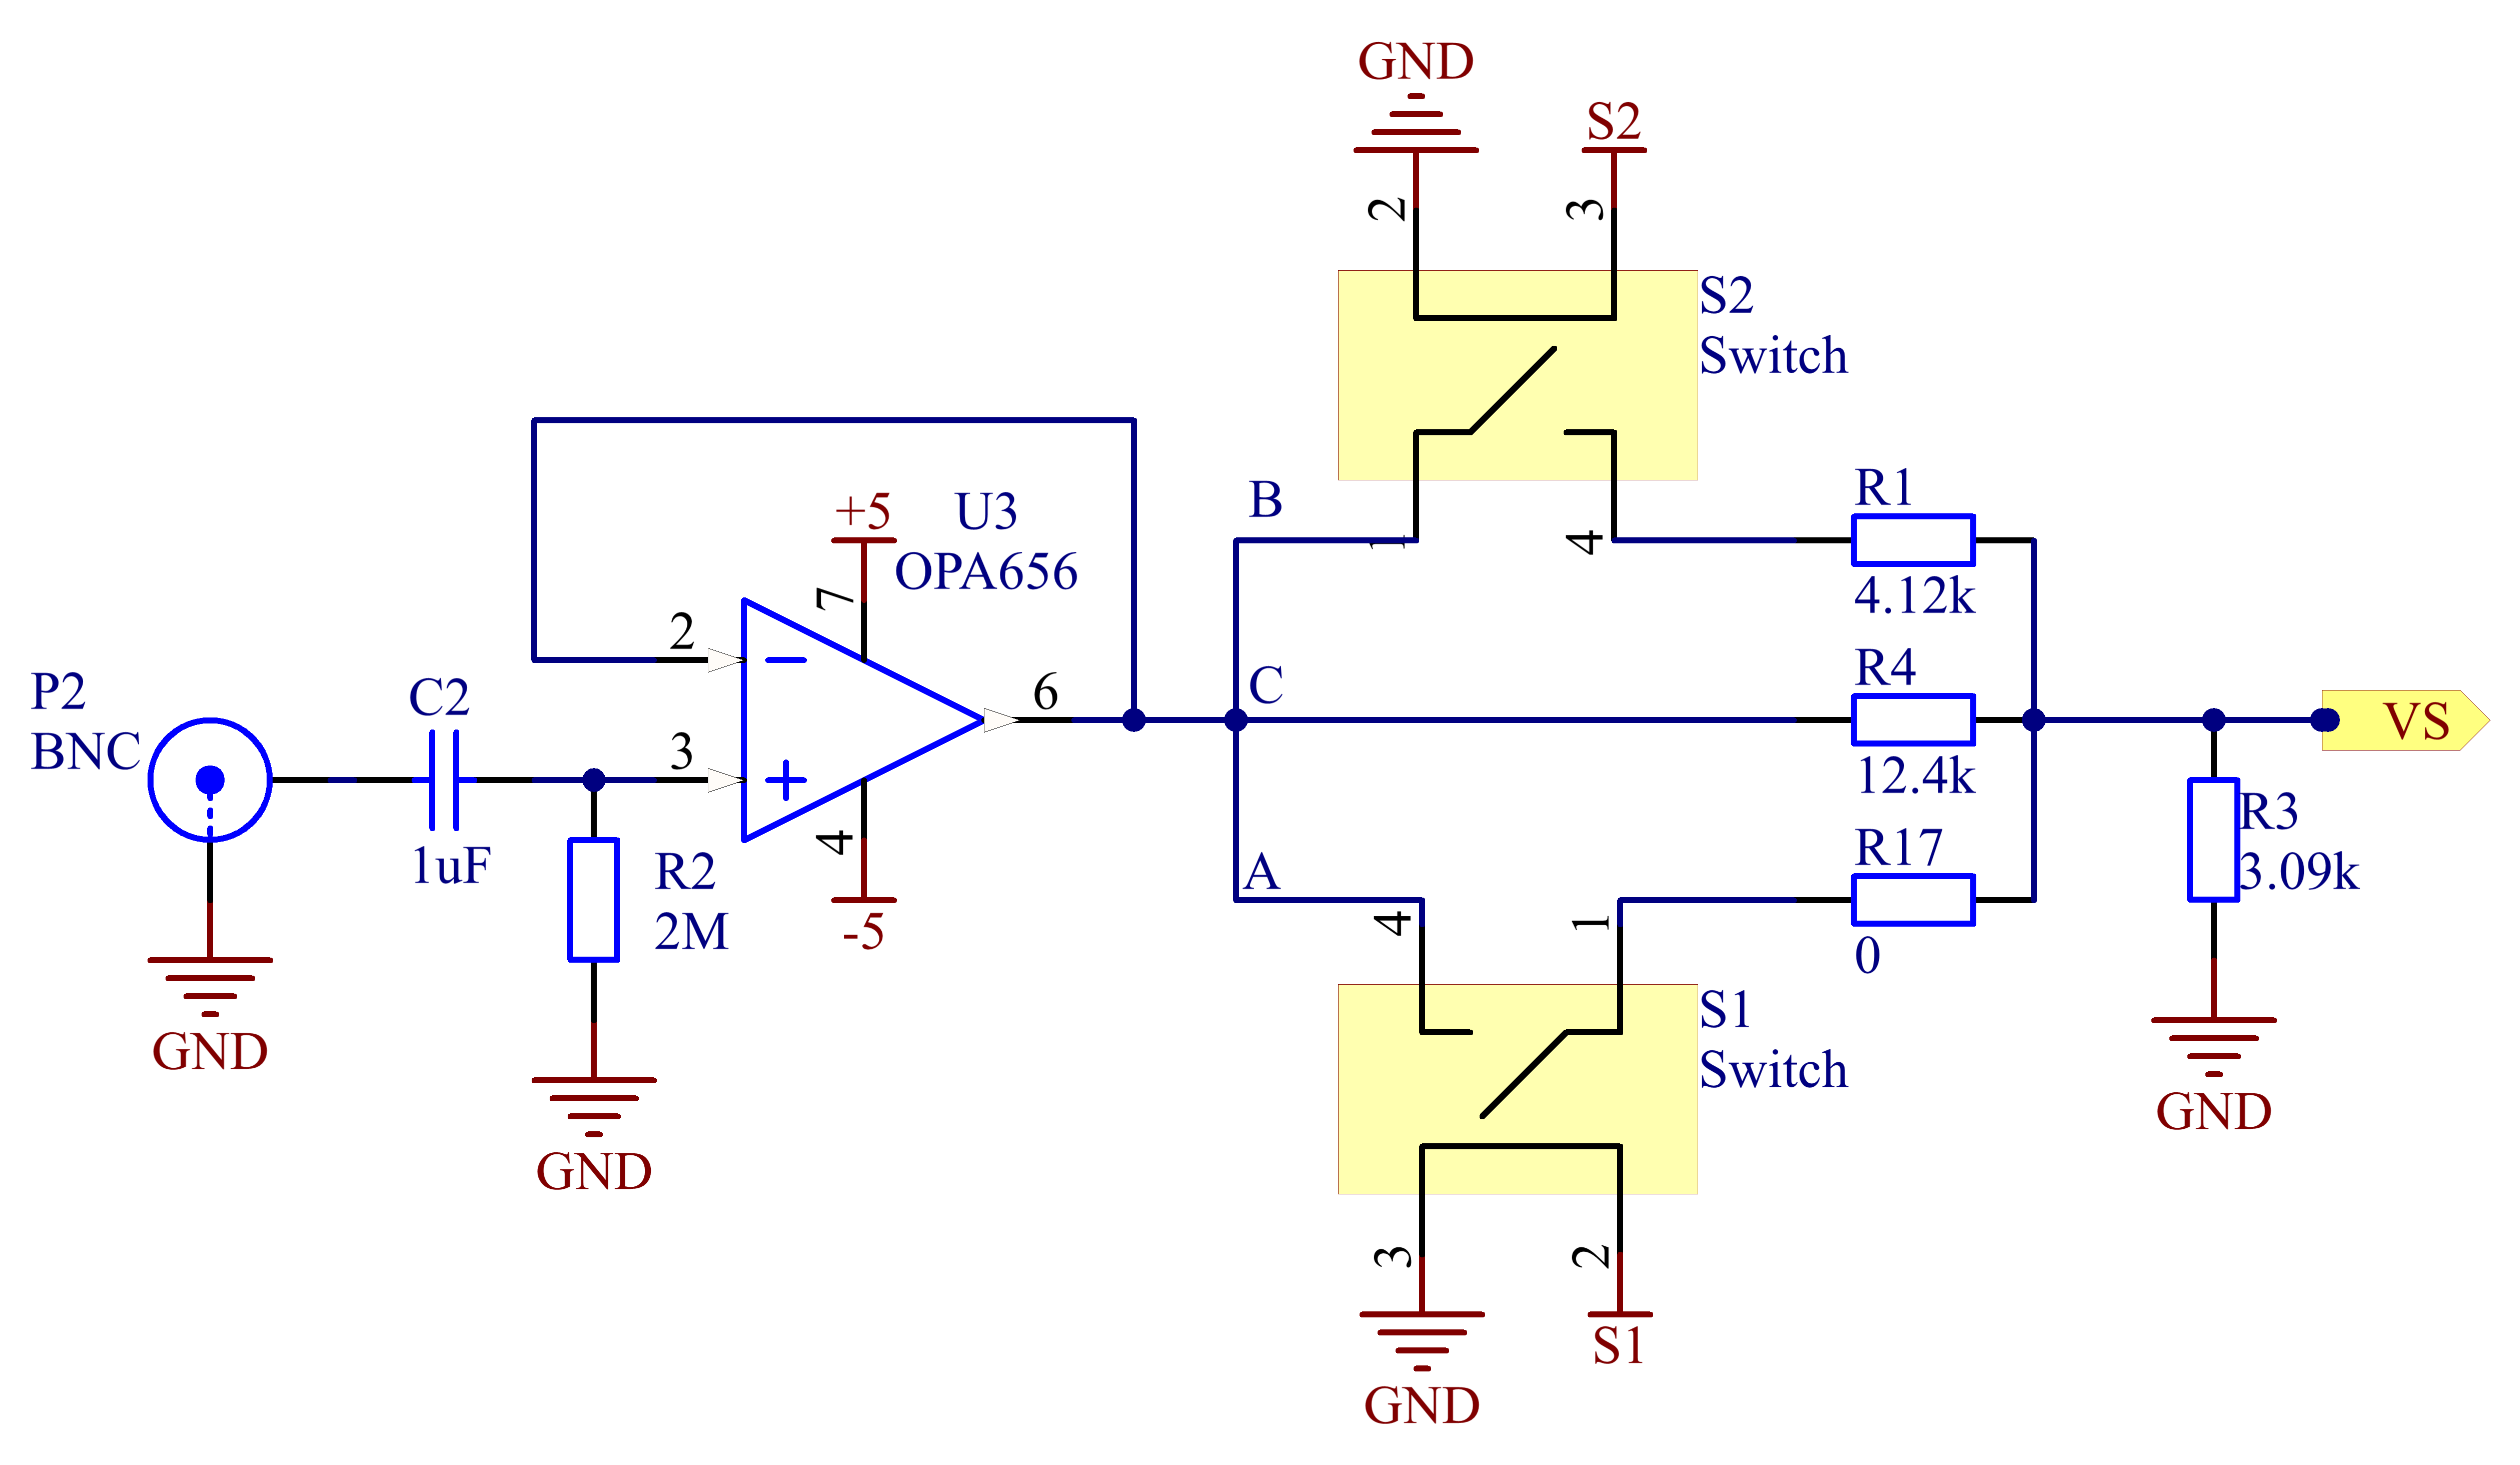
\includegraphics[width=10cm]{Figures/SwitchCircuit.png}
	\end{generalfig}
	
	抗混叠滤波电路选用五阶无源椭圆滤波器进行抗混叠滤波,使50MHz时信号衰减达到50dB,同时保证20MHz的有效信号输入范围。
	\begin{generalfig}[htb]{抗混叠滤波电路}{fig:FilterCircuit}
		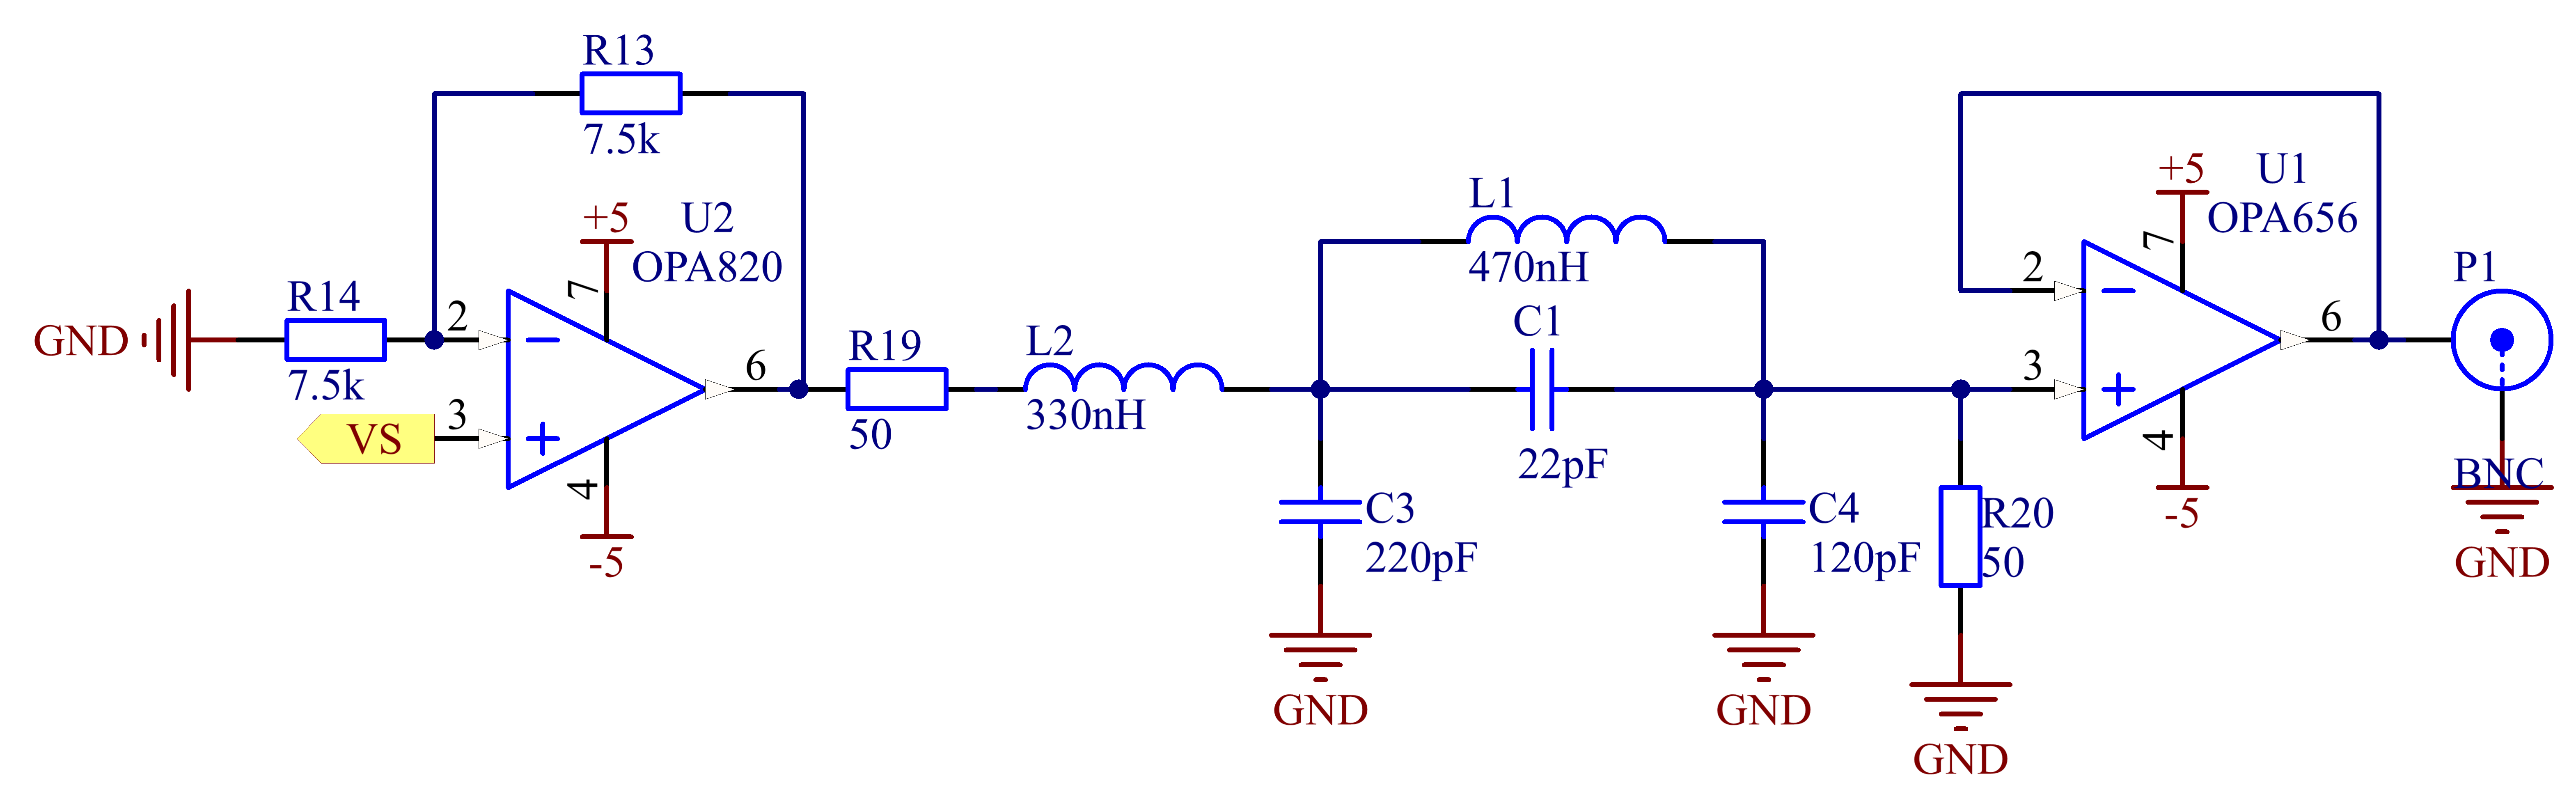
\includegraphics[width=12cm]{Figures/FilterCircuit.png}
	\end{generalfig}
	
	\subsection{高速ADC采样电路}
	
	选用ADI公司的8位双路高速模数转换器AD9288,其采样率最大可达100MSPS,可以满足题目要求。选用ADI公司的高速运算放大器AD8132将单端输入信号转成差分信号。
	\begin{generalfig}[htb]{ADC采样电路}{fig:ADCSamplingCircuit}
		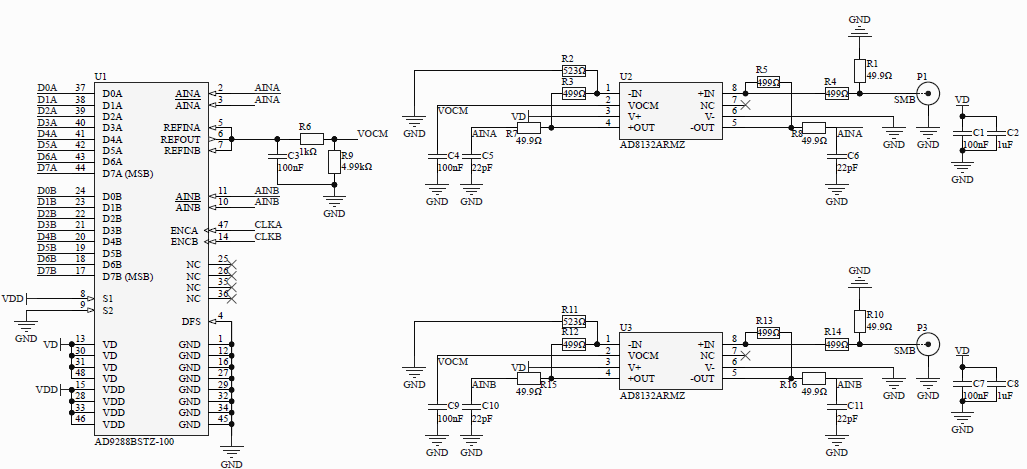
\includegraphics[width=\textwidth]{Figures/ADCSamplingCircuit.png}
	\end{generalfig}
	
	
	\subsection{电源设计}
	本系统使用了高精度高速ADC作为前级采样,要求电源有较高的稳定性,前级信号调理电路也对电源要求颇高。故设计了如\autoref{fig:LdoPower}所示的LDO稳压电路,得到纹波较小的±5V电压。经测试,本电源模块的纹波小于20mV。
	
	\begin{generalfig}[htb]{LDO电源模块电路}{fig:LdoPower}
		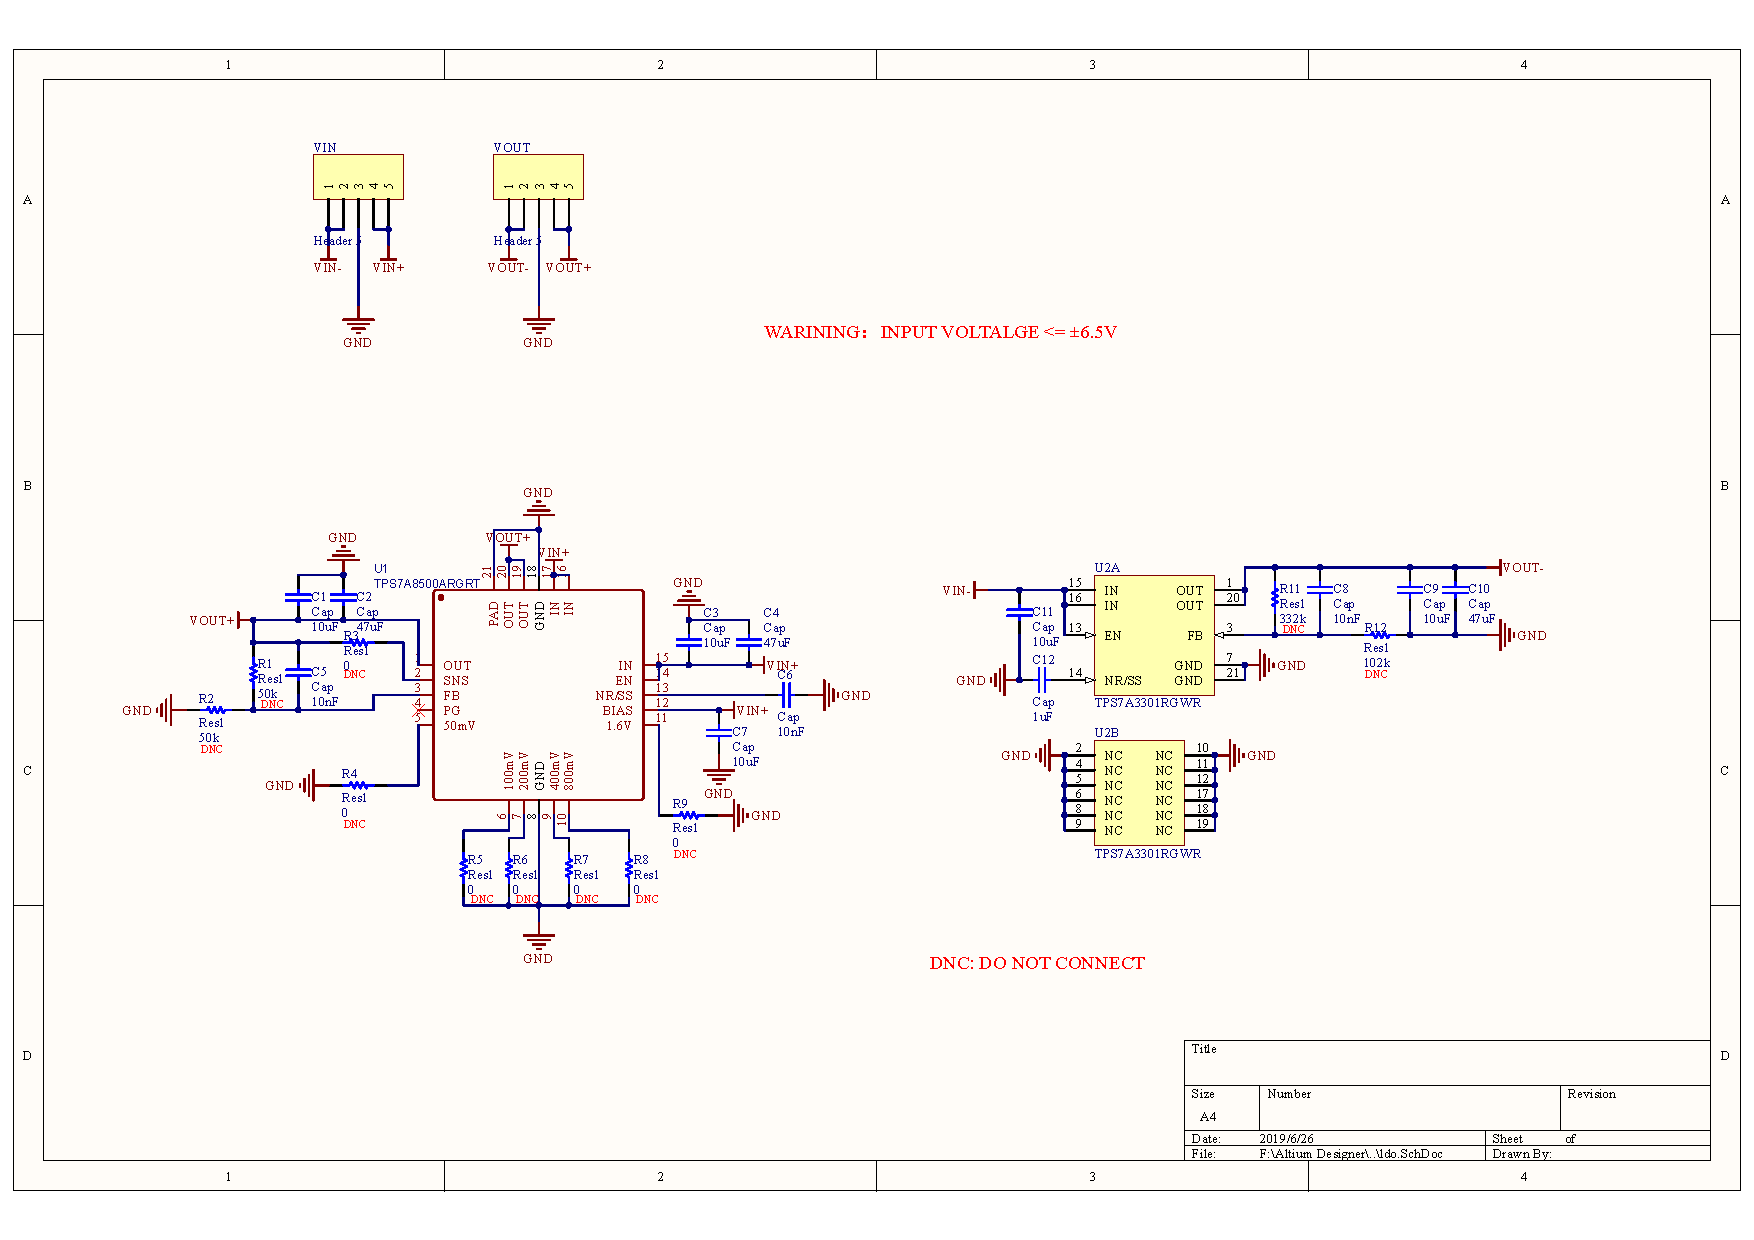
\includegraphics[width=14cm]{Figures/LdoPower.pdf}
	\end{generalfig}
	
	
	\section{程序设计}
	\subsection{PS-PL协同设计概述}
	本设计采用微雪7寸液晶显示屏来进行人机交互,该显示屏带有触摸功能,在检测到触摸时会触发I2C接口产生相应的信息,包含触摸点坐标等。因此,需要设计人机交互以及数据交互,故引入Zynq系列软硬件协同开发方案,即PS(Process System)-PL(Programmable Logic)交互,底层PL部分负责采样系统控制,顶层PS负责运行时调度、与PL数据交互以及与用户人机交互。
	
	\subsection{嵌入式软件开发}
	
	为了更方便地进行嵌入式软件部分开发,本设计移植了一套精美的嵌入式图形库Littlevgl。这套嵌入式图形库不仅利于开发嵌入式UI,还自带实时操作系统RTOS,即使不用嵌入式操作系统(即裸机开发),也可以很好地达到任务调度的目的。
	
	除此之外,该图形库还具有完善的API,方便进行调用,同时也有基于Eclipse开发的UI仿真环境,便于调试。图\autoref{fig:Software}为本设计的软件程序框图。
	
	
	\begin{generalfig}[htb]{软件程序框图}{fig:Software}
		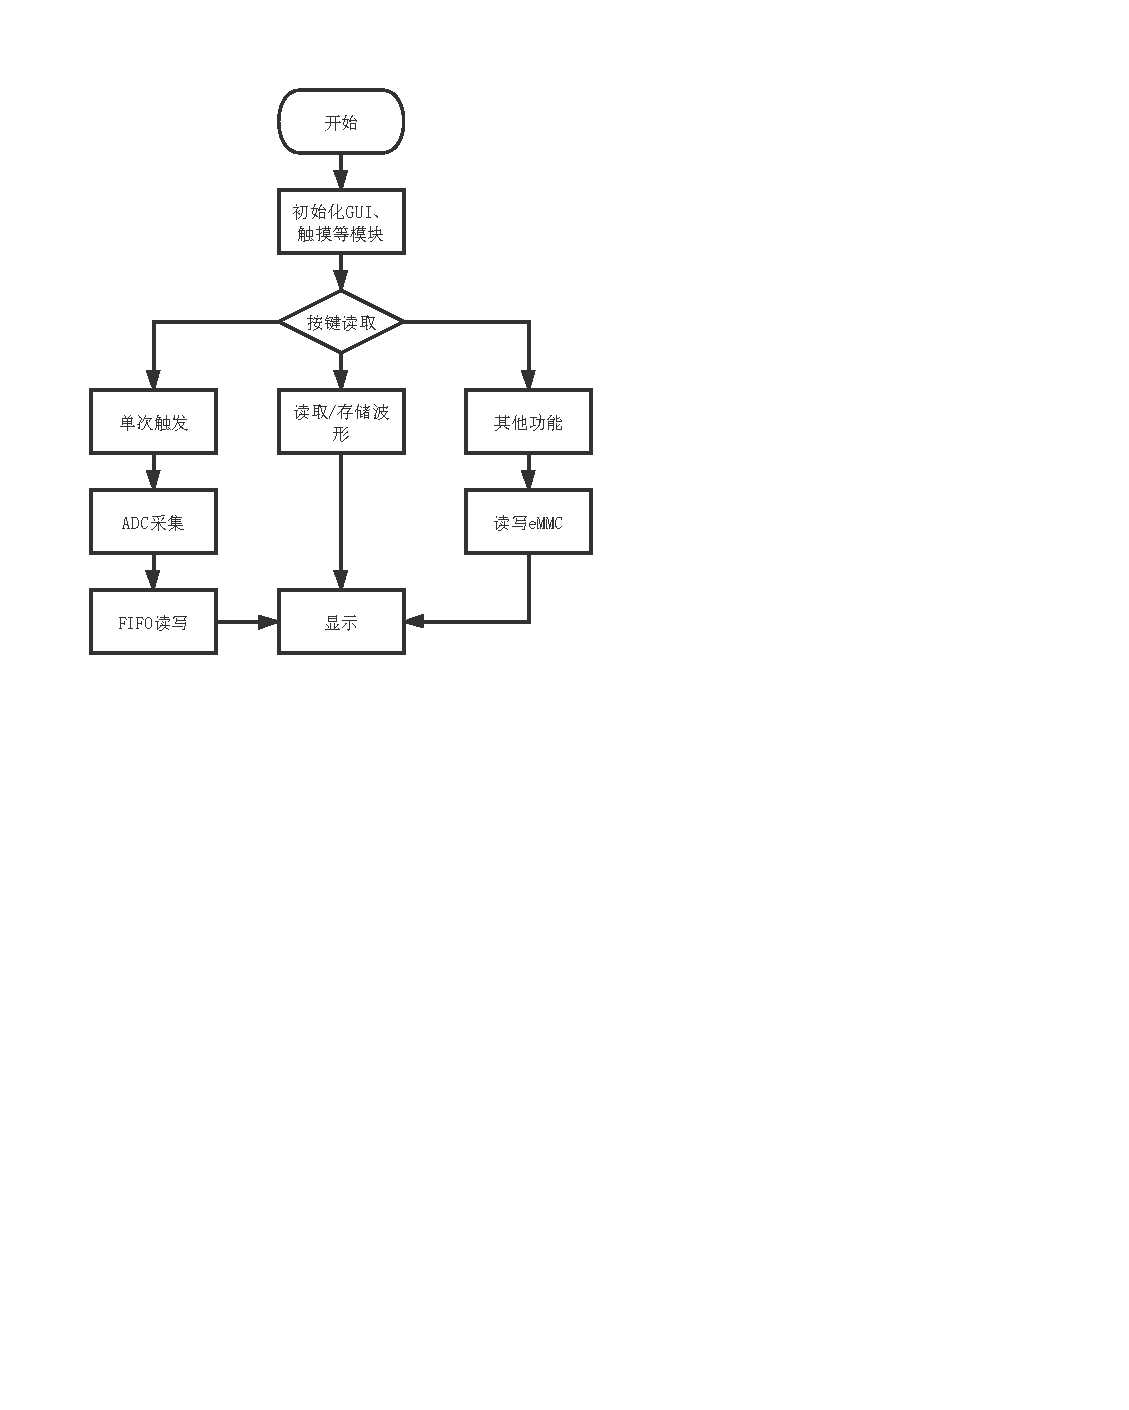
\includegraphics[width=8cm]{Figures/Software.pdf}
	\end{generalfig}

	
	\subsection{FPGA逻辑开发}
	如\autoref{fig:BlockDesign}所示即为本设计的软硬件协同开发模块互联图(Block Design),将示波器采样控制模块、PS部分、FIFO/DMA数据交互模块、VDMA/VTC显示控制部分全部整合到一起,实现了示波器采样控制、数据流控制、人机交互等功能整合开发。
	
	\begin{generalfig}[htb]{Block Design}{fig:BlockDesign}
		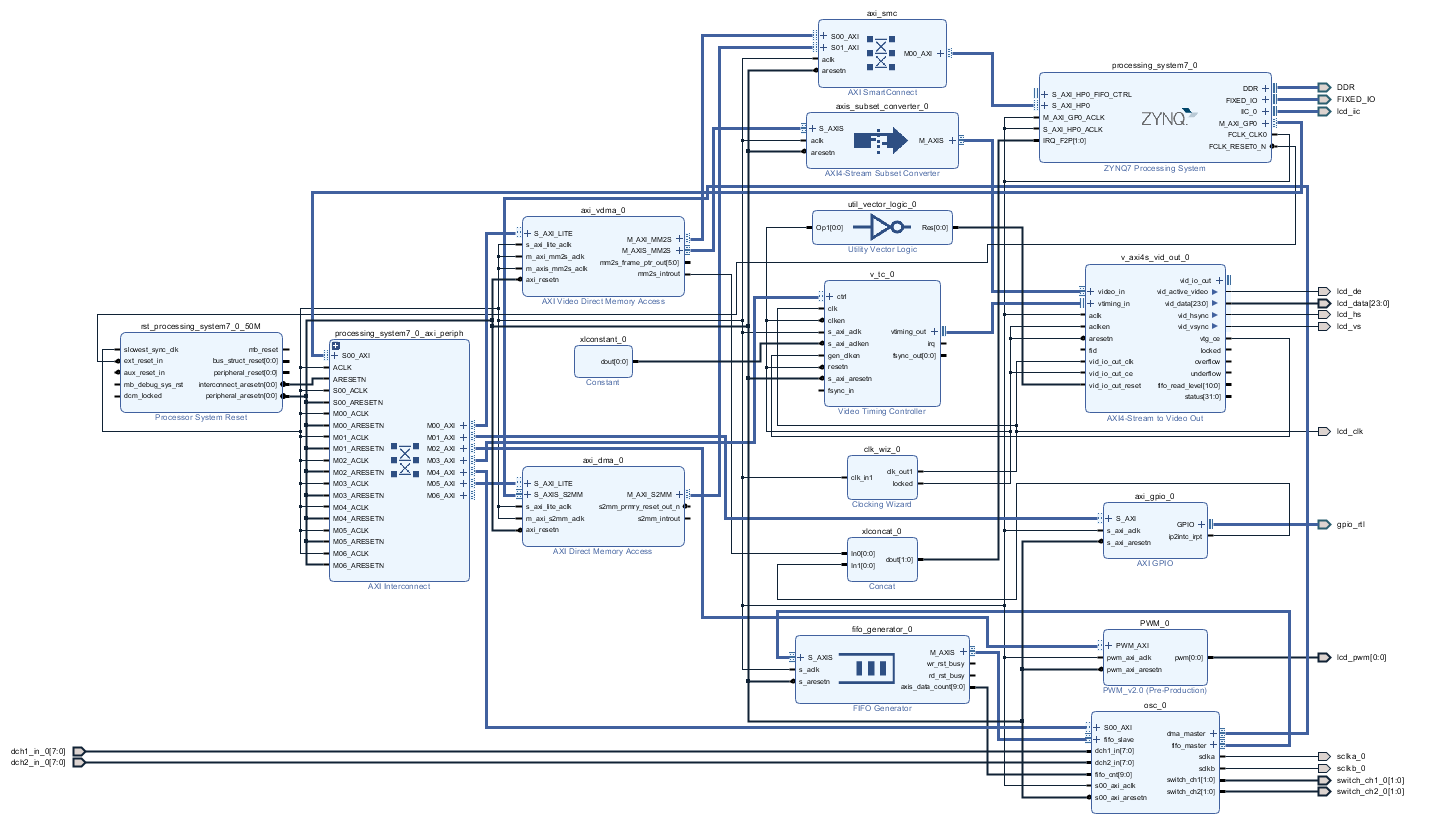
\includegraphics[width=\textwidth]{Figures/BlockDesign.png}
	\end{generalfig}
	
	下面分别介绍该作品使用到的PL部分模块,主要有FIFO模块、直接存储器访问(DMA)模块、液晶显示器驱动模块。
	
	\subsubsection{FIFO模块}
	FIFO模块使用Xilinx的IP进行配置,将数据宽度设置为4个字节,数据深度设置为512,提供余量以保证不会溢出,并且打开FIFO中已经存入的数据量计数接口,提供给触发采样状态机,满足状态转换进行的条件。相关配置如\autoref{fig:FIFOSetup}所示。
	
	\begin{generalfig}[htb]{FIFO配置}{fig:FIFOSetup}
		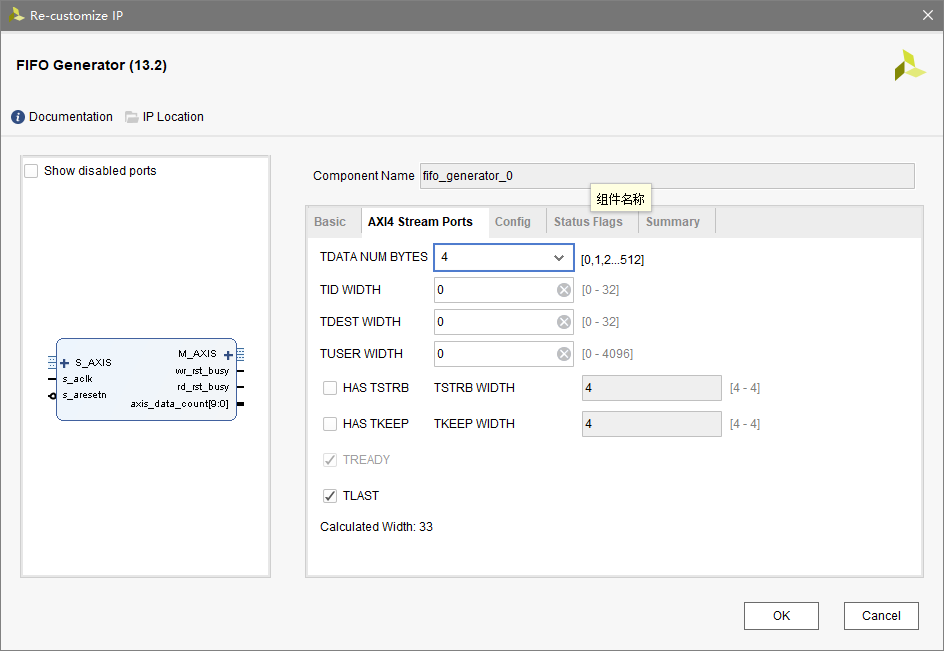
\includegraphics[width=12cm]{Figures/FIFOSetup.png}
	\end{generalfig}

	\subsubsection{直接存储器访问(DMA)模块}
	DMA使用Xilinx提供的IP进行配置,只需要其中的Write Channel即可。相关配置如\autoref{fig:DMASetup}所示。
	
	\begin{generalfig}[htb]{DMA配置}{fig:DMASetup}
		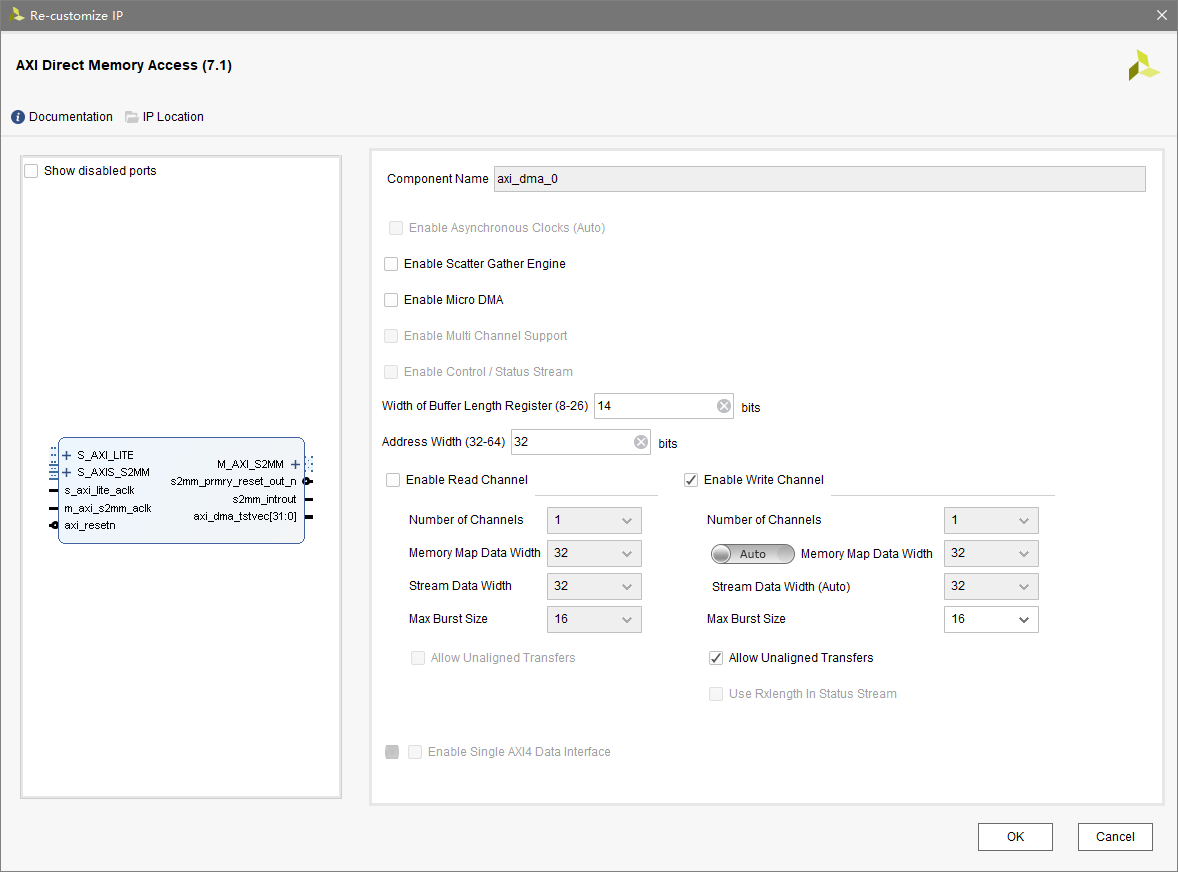
\includegraphics[width=12cm]{Figures/DMASetup.png}
	\end{generalfig}
	
	\subsubsection{ZYNQ7 Processing System}
	软硬件协同设计的核心在于PS硬核处理器,这也是Xilinx公司的Zynq系列器件优势所在,能够比较方便地配置ARM Cortex-A9处理器,在Block Design中添加ZYNQ7 Processing System,再对其进行配置即可,\autoref{fig:PSClkSetup}和\autoref{fig:PSDDRSetup}分别截取了内存以及时钟的配置。
	
	\begin{generalfig}[htb]{PS时钟配置}{fig:PSClkSetup}
		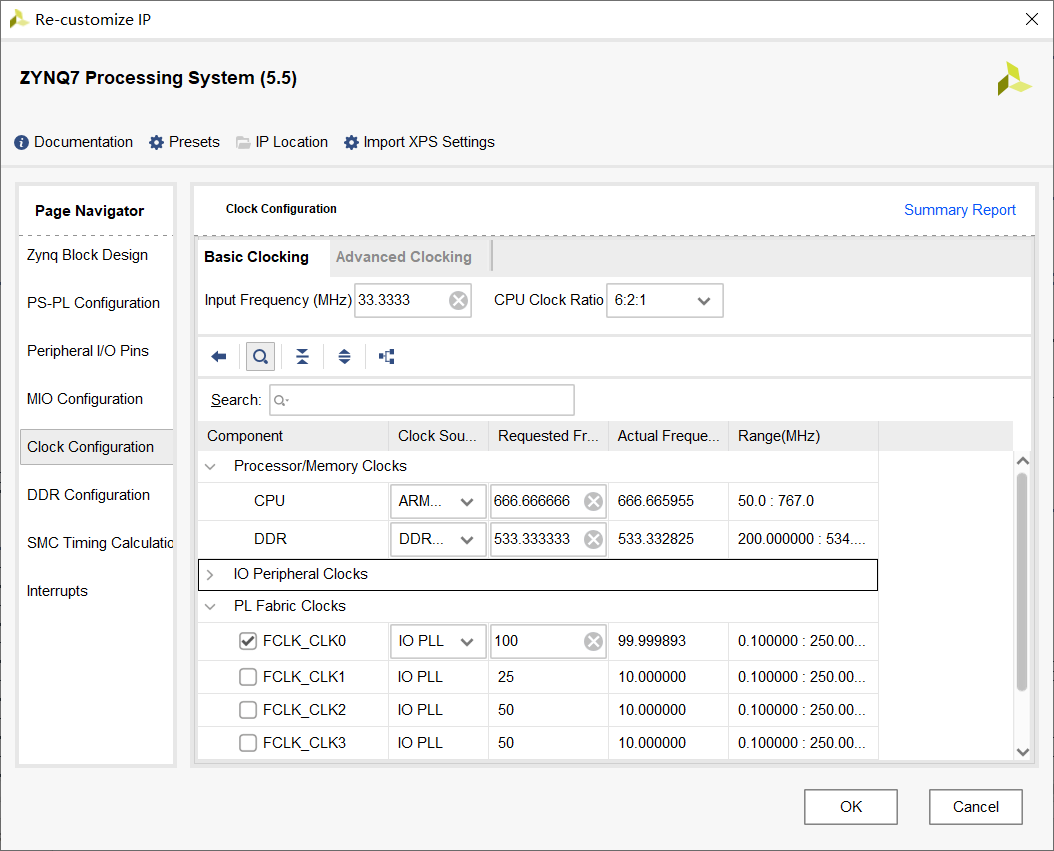
\includegraphics[width=12cm]{Figures/PSClkSetup.png}
	\end{generalfig}

	\begin{generalfig}[htb]{PS内存配置}{fig:PSDDRSetup}
		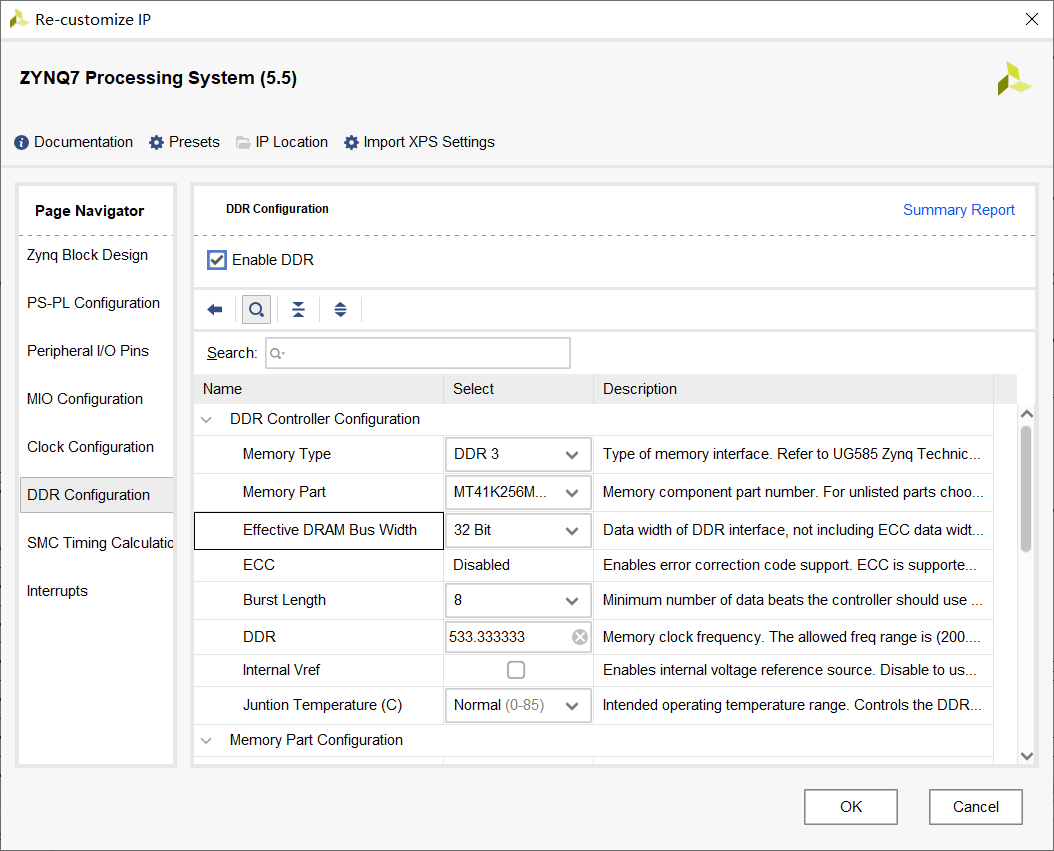
\includegraphics[width=12cm]{Figures/PSDDRSetup.png}
	\end{generalfig}
	
	
	\subsubsection{液晶显示器驱动模块}
	
	本系统使用了微雪公司的7寸液晶显示屏来显示界面,采用RGB并行数据传输的方式,通过视频流直接存储器访问(VDMA)模块来完成时序驱动。为了产生与数据流相匹配的时钟,我们采用了Xilinx公司的Video Timing Control IP核,与VDMA模块适配,完成场同步、帧同步等时序操作。该部分模块如\autoref{fig:VTCSetup}所示。
	\begin{generalfig}[htb]{Video Timing Control IP核配置}{fig:VTCSetup}
		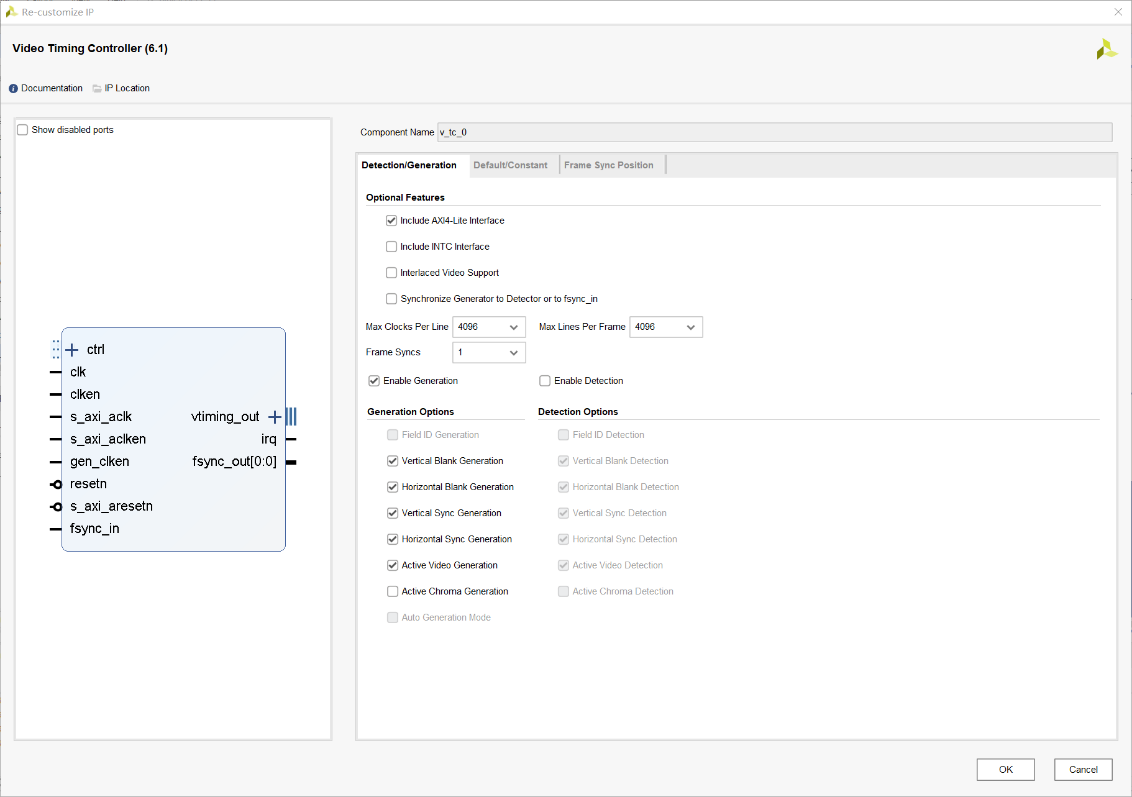
\includegraphics[width=12cm]{Figures/VTCSetup.png}
	\end{generalfig}
	
	打开VDMA的配置界面,如\autoref{fig:VDMASetup}所示,根据原理分析中的显示器时序图,我们可以配置出VDMA的参数,分辨率自定义,设置为我们使用的屏幕的1024×600分辨率。	
	\begin{generalfig}[htb]{Video DMA IP核配置}{fig:VDMASetup}
		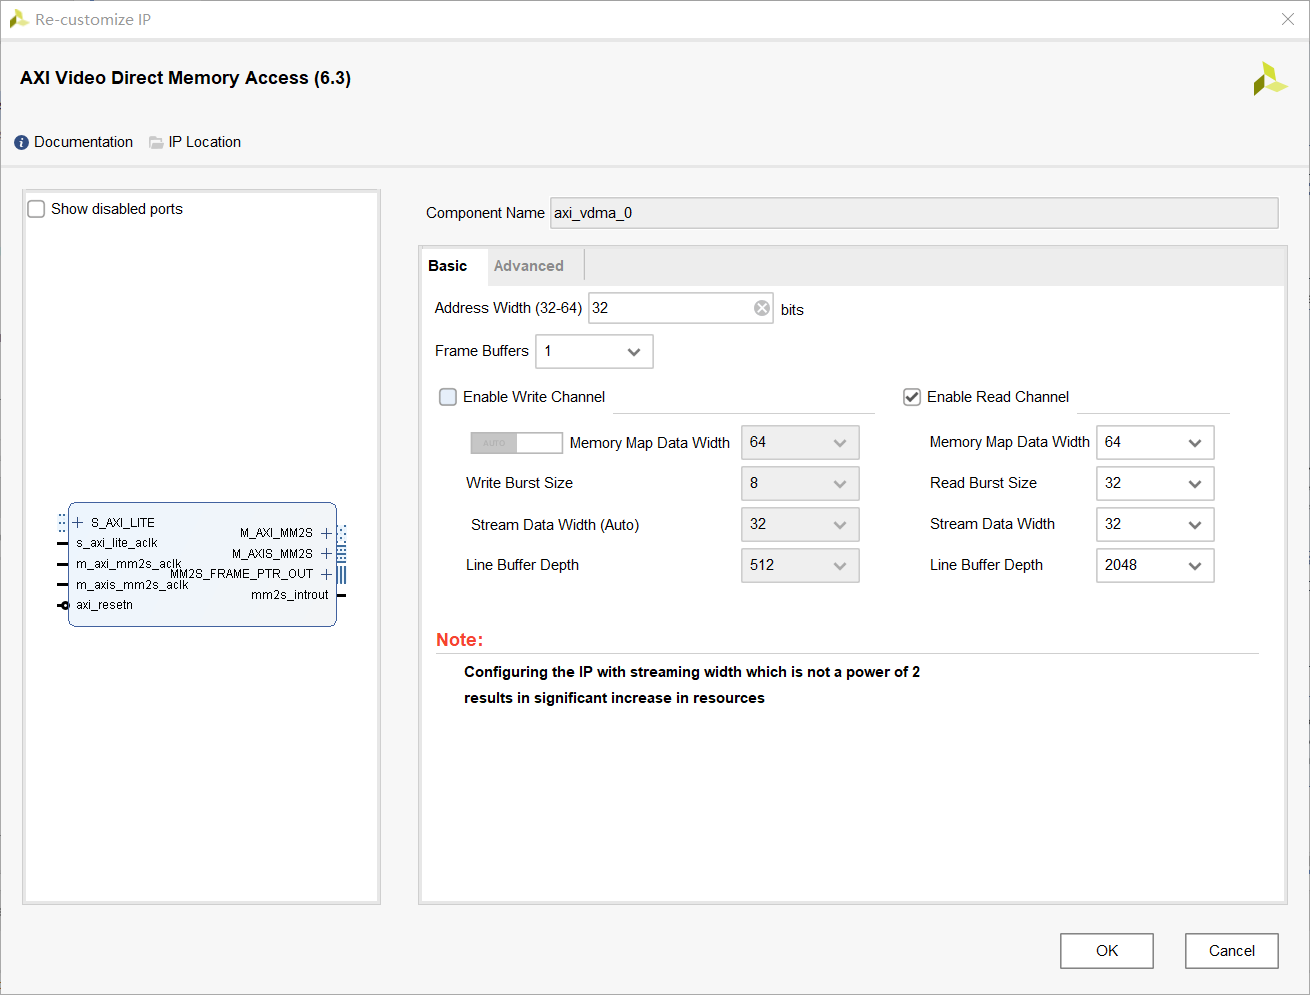
\includegraphics[width=12cm]{Figures/VDMASetup.png}
	\end{generalfig}

	打开Clocking Wizard的配置界面,如\autoref{fig:ClockingWizardSetup}所示,同理可得配置参数。注意要和VDMA的配置保持一致,否则将出现时序错误,显示器的驱动时钟为51.2MHz,所以这里要做相应的配置。
	\begin{generalfig}[htb]{锁相环配置}{fig:ClockingWizardSetup}
		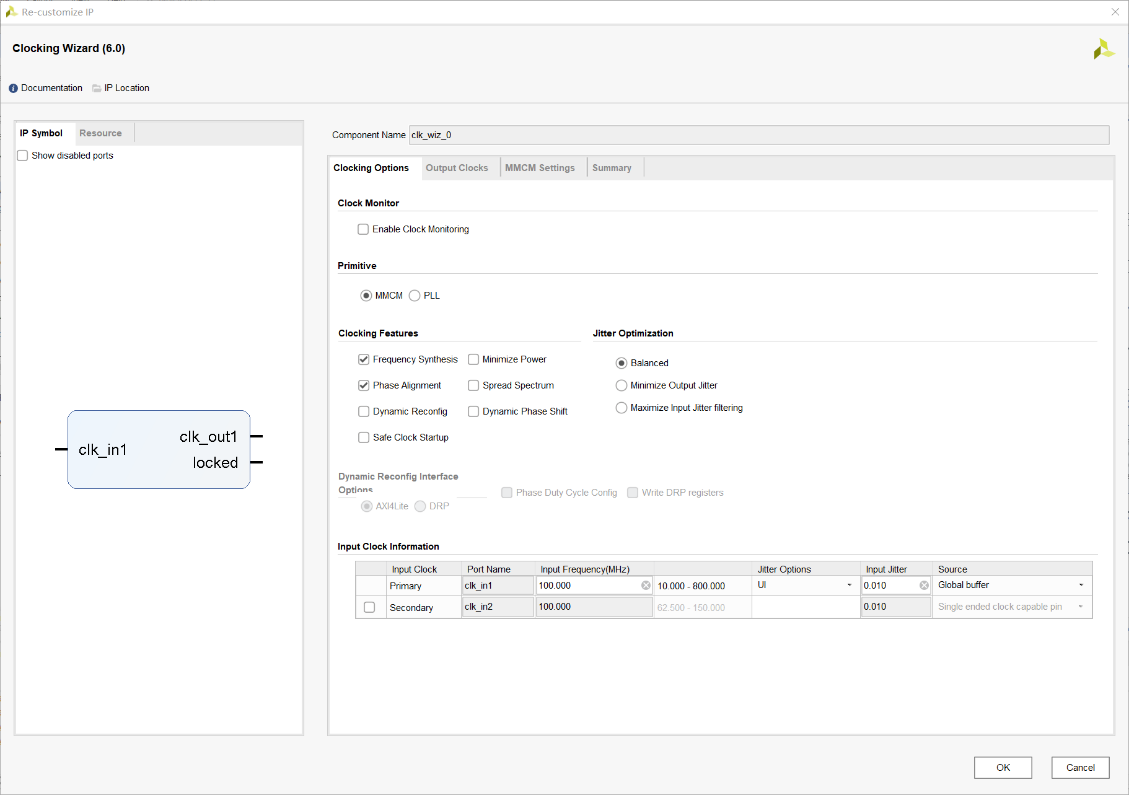
\includegraphics[width=12cm]{Figures/ClockingWizardSetup.png}
	\end{generalfig}
	
	最后,在连线时,VDMA和VTC之间需要做位宽桥接,调用Xilinx的IP核来完成位宽转换。在连线时,需要把锁相环的Lock信号连接到各个显示屏驱动相关IP核的使能接口上,保证在锁相环产生了稳定的时钟之后,再触发传输。
	
	如此便完成了液晶显示器驱动模块的设计,最后将配置好的RGB接口引出即可。整个显示器驱动模块的架构如\autoref{fig:DisplayModule}所示。
	\begin{generalfig}[htb]{显示器驱动模块的架构图}{fig:DisplayModule}
		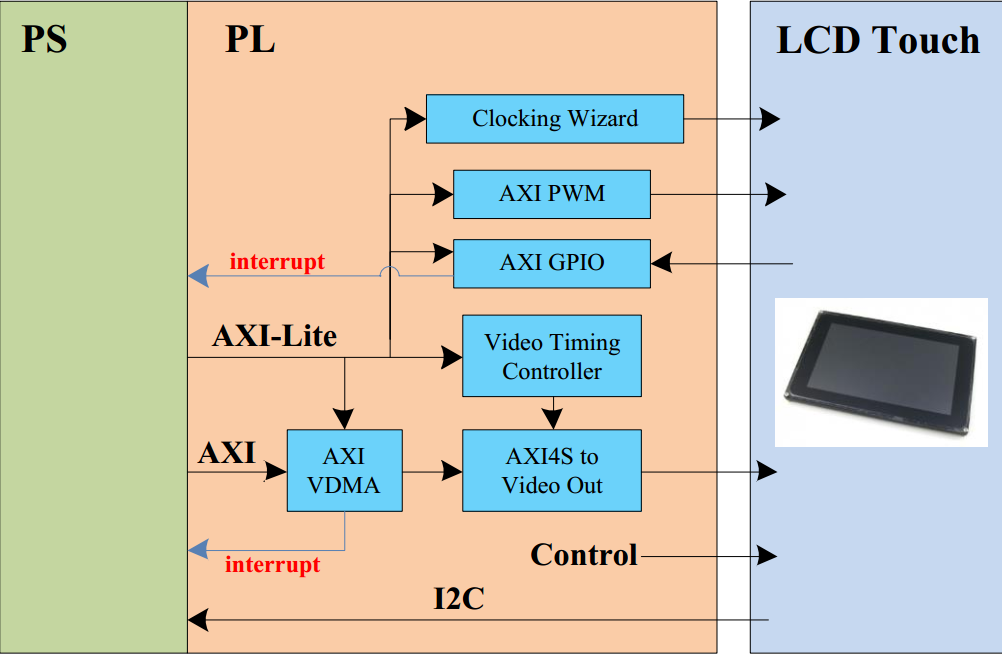
\includegraphics[width=12cm]{Figures/DisplayModule.png}
	\end{generalfig}
	
	
	\section{系统仿真与调试}
	
	\subsection{FPGA开发流程}
	
	\subsubsection{开发流程重要步骤说明与图示}
	
	\subsubsubsection{新建工程}
	进入Vivado开发平台后,首先点击新建工程,如\autoref{fig:NewProject}所示。
	
	\begin{generalfig}[htb]{新建工程}{fig:NewProject}
		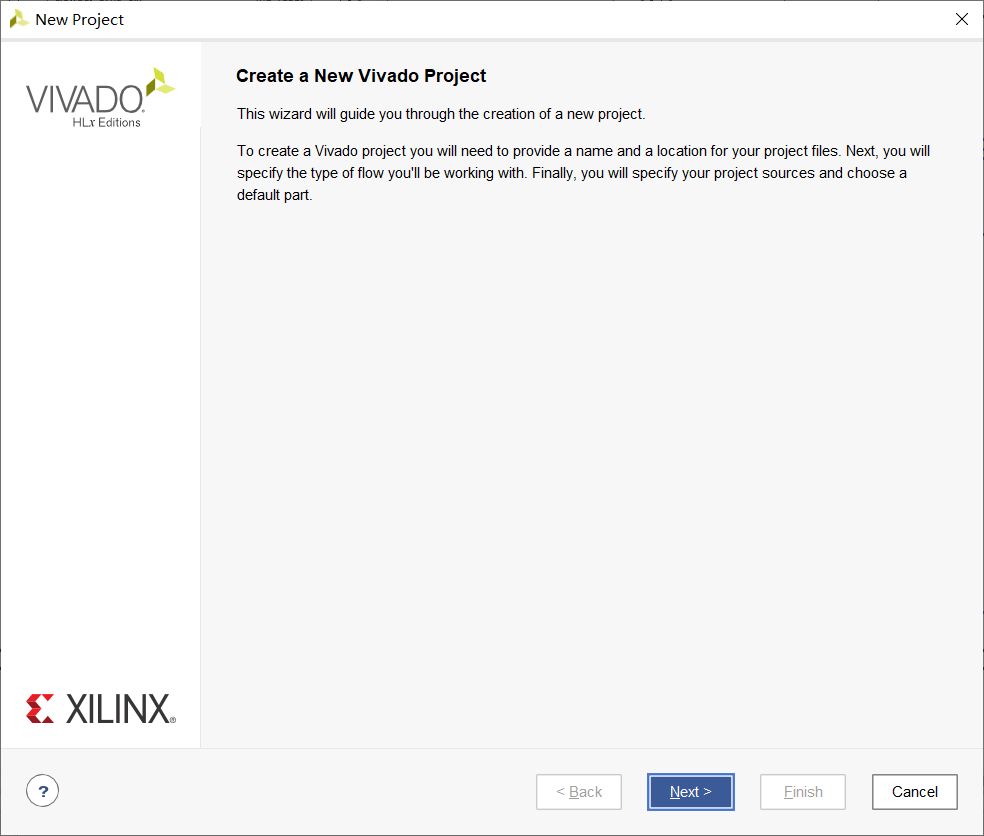
\includegraphics[width=12cm]{Figures/NewProject.png}
	\end{generalfig}
	
	
	确定工程的名字和路径之后,下一步是器件选型,本课程设计选用的FPGA型号为Zynq-7020,因此芯片型号为xc7z020clg400-2,如\autoref{fig:PartChoose}所示。
	
	\begin{generalfig}[htb]{器件选型}{fig:PartChoose}
		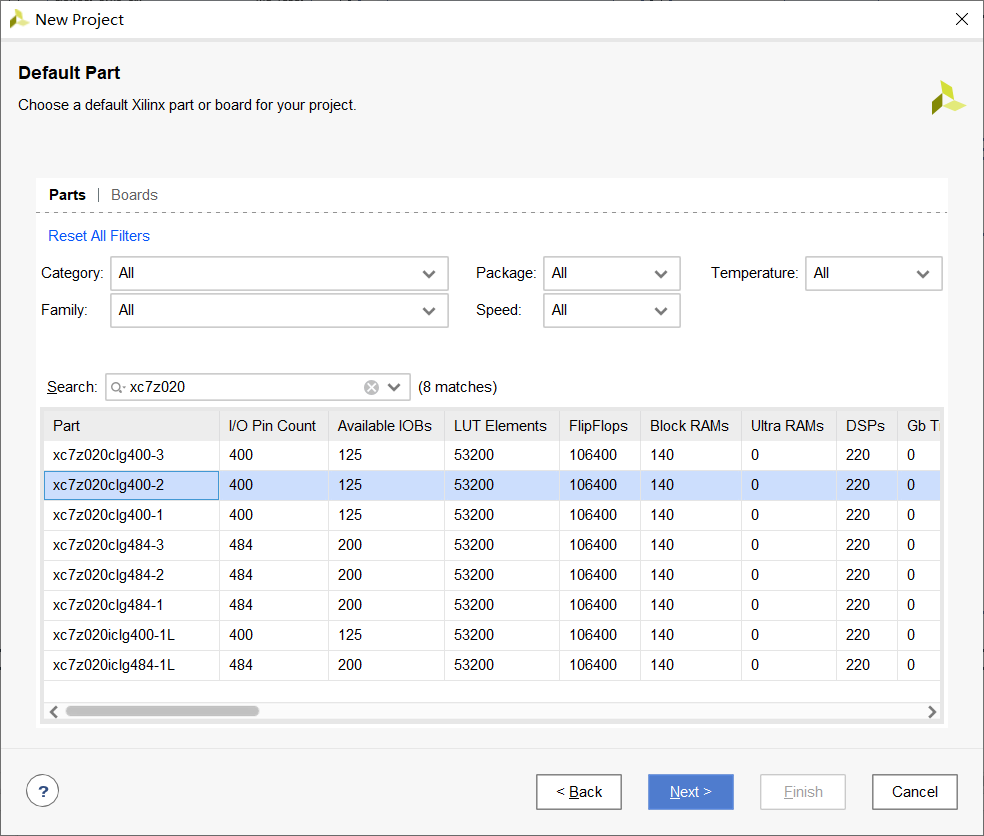
\includegraphics[width=12cm]{Figures/PartChoose.png}
	\end{generalfig}

	配置好器件型号之后,即完成了工程的创建,如\autoref{fig:FinishCreate}所示。
	
	\begin{generalfig}[htb]{完成创建}{fig:FinishCreate}
		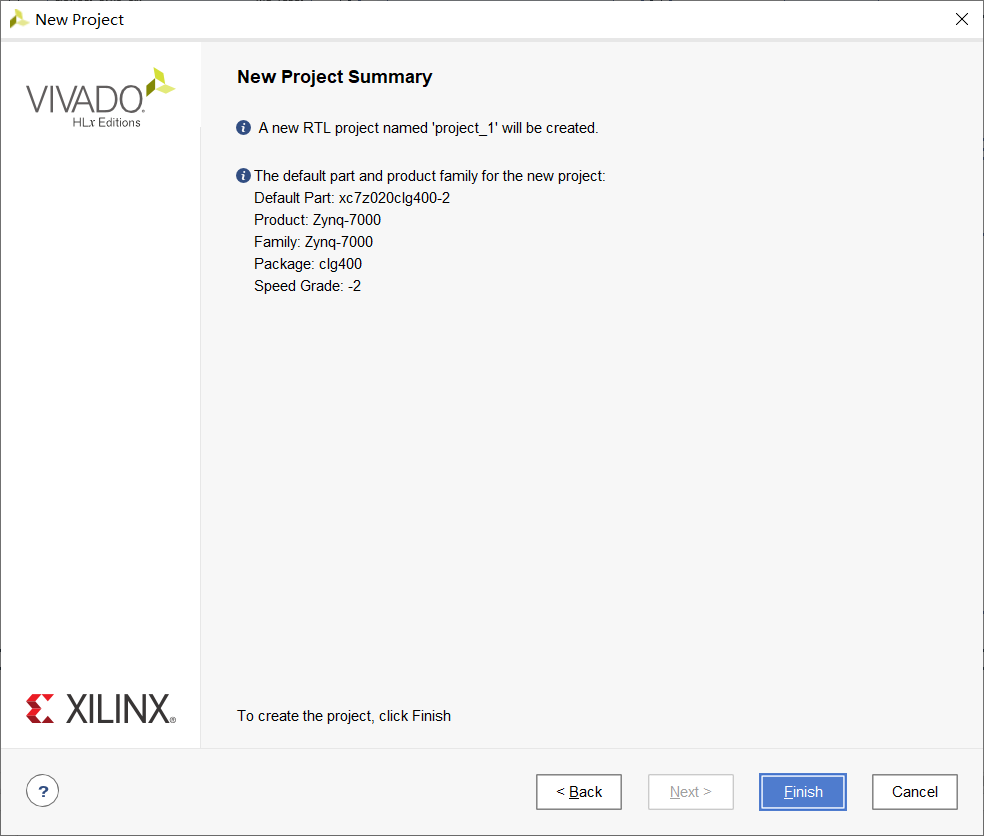
\includegraphics[width=12cm]{Figures/FinishCreate.png}
	\end{generalfig}

	\subsubsubsection{新建文件}
	进入新的Vivado工程之后,我们选择添加Block Design,因为本系统是软硬件协同的,需要用到处理器,因此选用Block Design模块化设计,如\autoref{fig:CreateBlockDesign}所示。
	
	\begin{generalfig}[htb]{添加Block Design}{fig:CreateBlockDesign}
		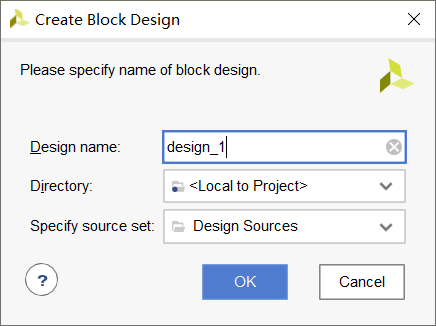
\includegraphics[width=8cm]{Figures/CreateBlockDesign.png}
	\end{generalfig}
	
	
	
	添加好之后即添加IP、配置IP并连线、输出等等,完成后的设计图在上文中提到。选择让Vivado自动生成顶层Verilog代码,即可完成硬件部分的逻辑设计,顶层Wrapper将会自动生成。
	
	\subsubsubsection{功能仿真}
	在设计每一个模块时,需要对模块进行功能仿真,Xilinx的Vivado平台自带仿真系统,也可以使用业界常用的Modelsim进行仿真。本设计使用Vivado进行综合前仿真,以验证功能正确性。
	
	编写testbench时,使用DDS(Direct Digital Synthesis,直接数字频率合成)生成模拟的正弦信号作为仿真信号源给状态机进行仿真。仿真模块实例化触发状态机以及FIFO,DMA部分由于缺少与处理器的交互没有加入仿真验证。经过修改验证,得到如\autoref{fig:VivadoSim}所示的正确的仿真波形。
	
	\begin{generalfig}[htb]{Vivado功能仿真}{fig:VivadoSim}
		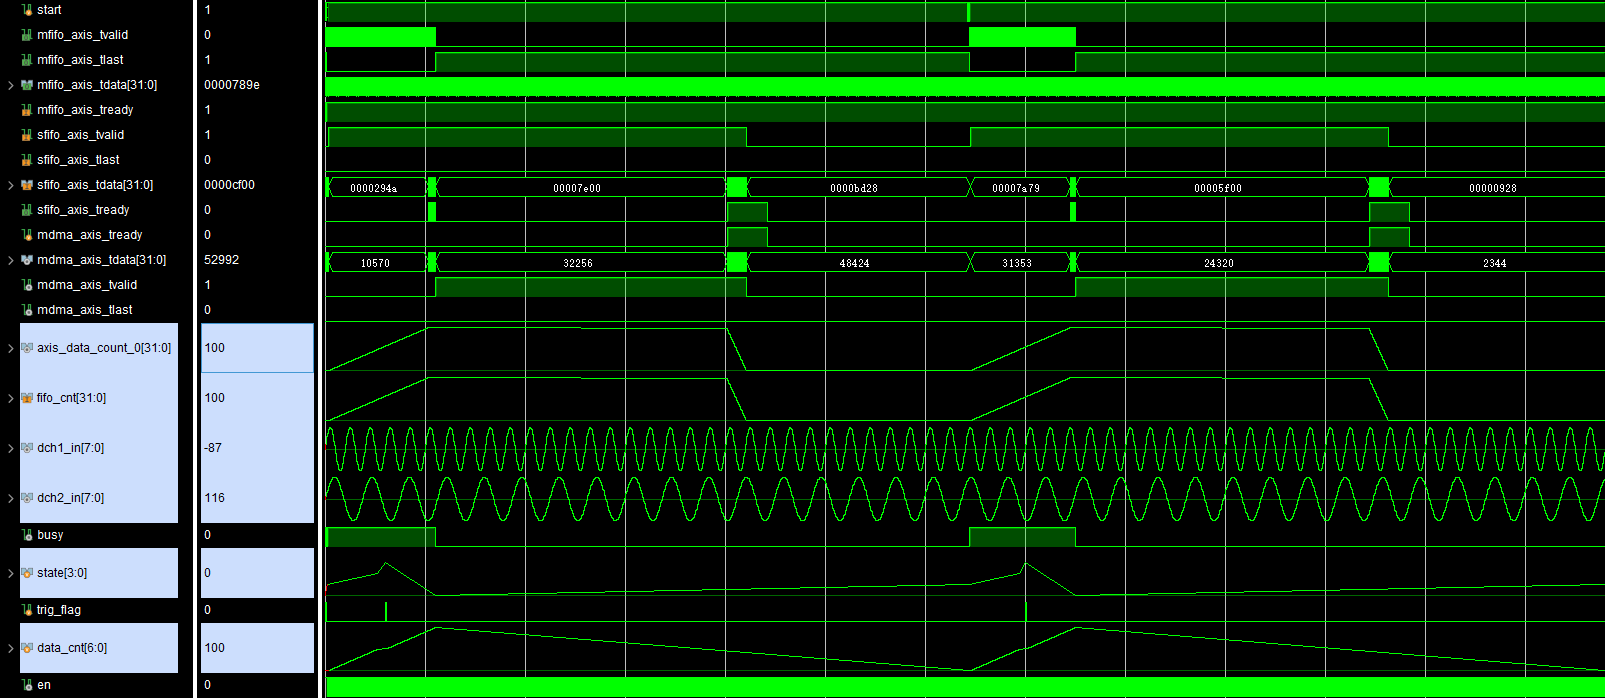
\includegraphics[width=12cm]{Figures/VivadoSim.png}
	\end{generalfig}	
	
	\subsubsubsection{引脚约束}

	使用直接编写约束文件的方式,能大大提高开发效率,因为可以通过模板来快速编写约束文件,如\autoref{fig:XDCFile}所示为节选的约束文件。
	
	\begin{generalfig}[htb]{引脚约束文件}{fig:XDCFile}
		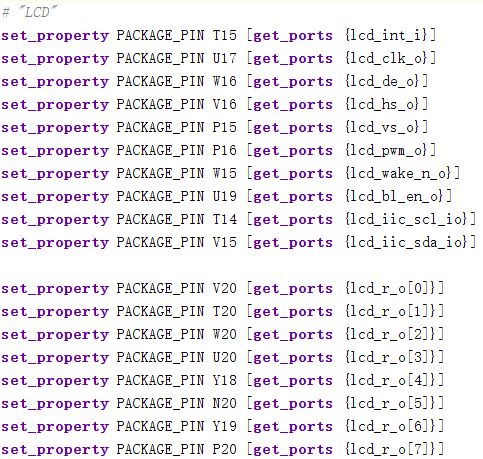
\includegraphics[width=8cm]{Figures/XDCFile.png}
	\end{generalfig}
	
	\subsubsubsection{时序约束}

	使用Vivado进行开发时,一般的时序约束方法有三种。
	
	{\songti \bfseries 方法1:自动创建基时钟和 PLL 输出时钟}
	
	
	这一方法能够自动地约束PLL的输入和输出时钟。ALTPLL mega function 中指定的所有 PLL 参数都用于约束 PLL 的输入和输出时钟。自动更新了 ALTPLL mega function的修改。当创建 PLL 的输入和输出时钟时,不必跟踪 PLL 参数的更改或指定正确的值。为了自动约束所有输入和输出,要将 derive\_pll\_clocks 命令和 -create\_base\_clocks选项一起使用。
	
	{\songti \bfseries 方法2:手动创建基时钟和自动创建 PLL 输出时钟}
	
	
	通过这种方法, 可以手动约束 PLL 的输入时钟并且使 TimeQuest analyzer 能够自动约束 PLL 的输出时钟。除此之外,与ALTPLL mega function 中指定的输入时钟频率相反,可以指定一个不同的输入时钟频率。通过使用 ALTPLL mega function 中指定的参数自动创建 PLL 输出时钟。
	
	{\songti \bfseries 方法3:手动创建基时钟和 PLL 输出时钟}
	
	
	通过这种方法,可以手动约束 PLL 的输入时钟和输出时钟。指定了所有的 PLL 参数并且参数值可以不同于 ALTPLL mega function 中指定的参数值。除此之外,可以尝试各种 PLL 输入和输出频率以及参数。也可以将该方法与 create\_clock 和 create\_generate\_clock 命令的组合一起使用。
	由于软硬件协同设计中,PL部分的时钟由PS内的锁相环提供,因此无需在约束文件中对PL时钟做过多约束。
	
	
	\subsubsubsection{综合RTL电路图}
	
	设计完成后,便可以进行综合,如果需要在线调试,还需要在综合结束之后进行配置以形成ILA。\autoref{fig:RTLFigure}是设计综合后的RTL电路图。
	
	\begin{generalfig}[htb]{RTL电路图}{fig:RTLFigure}
		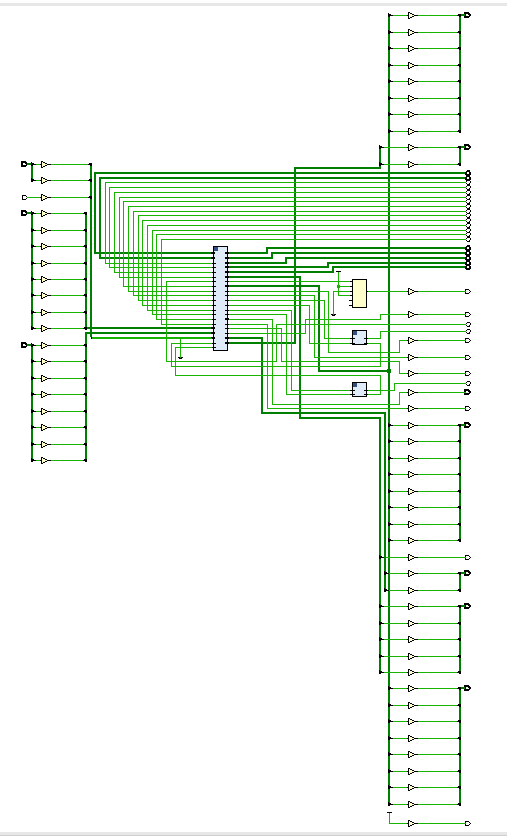
\includegraphics[width=8cm]{Figures/RTLFigure.png}
	\end{generalfig}
	
	\subsubsection{综合实现报告与分析}
	
	Verilog HDL是一种硬件描述语言,其最终的目的是生成硬件电路,所以与C语言不同,编程时特别在意硬件资源的消耗、时序分析以及功耗分析,如果实现相同的功能,而硬件消耗过多的话,那么这个设计就基本上是失败的。同理,时序、功耗等参数也是分析设计的重点。
	
	\subsubsubsection{时序报告分析}
	
	在一个时序电路中,一定要满足信号的建立时间和保持时间,否则信号时序出错,数据不能正确的传达。
	
	根据在数字电路基础这门课上学到的知识,可以得到以下的参数关系。
	
	{\songti \bfseries 建立时间}(Ts:set up time)是指在时钟沿到来之前数据从不稳定到稳定所需的时间,如果建立时间不满足要求,那么数据将不能在这个时钟上升沿被稳定地送入触发器;{\songti \bfseries 保持时间}(Th:hold time)是指数据稳定后保持的时间,如果保持时间不满足要求那么数据同样也不能被稳定地送入触发器。
	
	由于建立时间与保持时间的和是稳定的一个时钟周期,如果时钟有延时,同时数据的延时也较小,那么建立时间必然是增大的,保持时间就会随之减小,如果减小到不满足D2的保持时间要求时就不能采集到正确的数据,这时即$ T-(T_{pd}-T_{co}-T_{2min})< T_4 $,就不满足要求了,所以D2的保持时间应该为:$ T-(T_{pd}+T-T_{co}-T_{2min})\ge T_4 $即$ T_{co}+T_{2min} - T_{pd} \ge T_4 $从上式也可以看出如果$ T_{pd}=0 $也就是时钟的延时为0,那么同样要求$ T_{co}+T_{2min}>T_4 $,但是在实际的应用中由于$ T_2 $的延时也就是线路的延时远远大于触发器的保持时间即$ T_4 $,所以不必要关心保持时间。
	
	\autoref{fig:TimingReport}为时序分析报告,可以看到,在100MHz时钟下,建立时间、保持时间以及脉宽都满足时序约束要求。
	
	\begin{generalfig}[htb]{时序分析报告}{fig:TimingReport}
		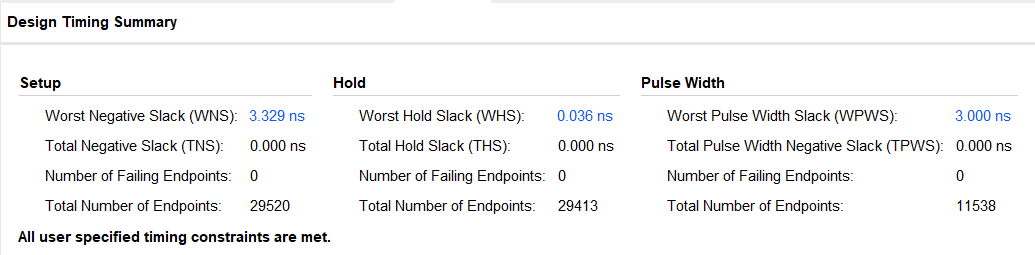
\includegraphics[width=\textwidth]{Figures/TimingReport.png}
	\end{generalfig}
	
	\subsubsubsection{功耗分析}
	
	低功耗是集成电路发展的一个趋势,如果实现一个完好的功能,实现了较低的功耗,那么这样的产品无疑是极有竞争力的。因此需要研究系统功耗,在Xilinx的集成开发工具Vivado中,带有功耗分析的功能。\autoref{fig:PowerAnalysis}所示为系统的功耗分析报告。
	
	\begin{generalfig}[htb]{功耗分析报告}{fig:PowerAnalysis}
		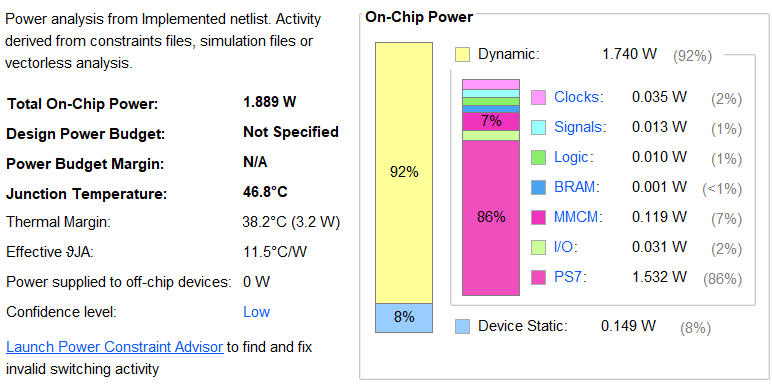
\includegraphics[width=12cm]{Figures/PowerAnalysis.png}
	\end{generalfig}
	
	从图中可以看出,本设计的功耗主要用在ARM核上(即PS部分),达到了总功耗的86\%。本设计使用了很多数据传输的IP核,这些IP核都是需要高速时钟驱动的,而逻辑部分没有占用太多的功耗,可以说本系统在功耗上控制得不错。
	
	\subsubsubsection{资源分析}
	从综合到实现,Vivado工具会帮我们做一些布局布线的优化,所以综合阶段的资源占用和实现阶段的资源占用是不一样的,因此选用实现阶段后的资源报告来作为最终的资源分析,如\autoref{fig:ResourceAnalysis}所示。
	
	\begin{generalfig}[htb]{资源分析}{fig:ResourceAnalysis}
		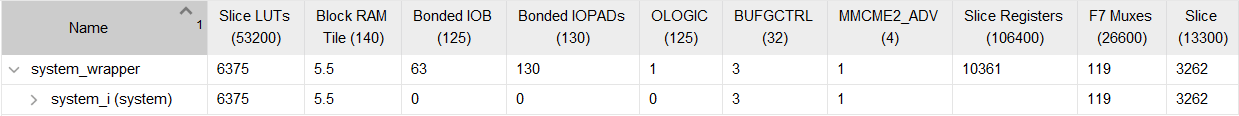
\includegraphics[width=\textwidth]{Figures/ResourceAnalysis.png}
	\end{generalfig}
	
	\subsubsubsection{电路实现版图}

	如\autoref{fig:FPGAFinalFig}所示为我们作品的最终FPGA版图。
	
	
	\begin{generalfig}[htb]{FPGA实现版图}{fig:FPGAFinalFig}
		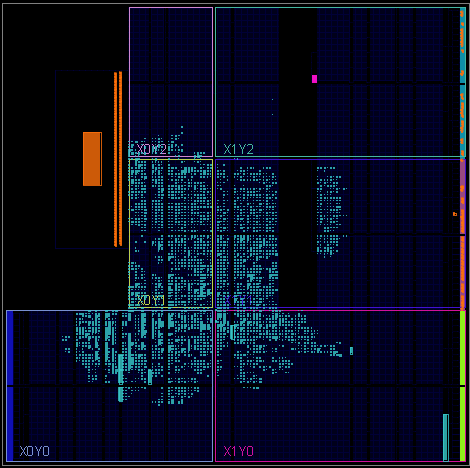
\includegraphics[width=12cm]{Figures/FPGAFinalFig.png}
	\end{generalfig}

	可以看到,版图中用于实现逻辑的部分不算多,且逻辑占用大多用于通用的FIFO、DMA、VDMA等数据传输模块。众所周知,越通用的IP越会占用更多的资源去完成通用性,因此选用Xilinx的通用IP核只是为了提高开发效率,它会占用更多的资源。
	
	\subsection{FPGA调试}
	
	\subsubsection{ILA测试简介}
	
	\subsubsubsection{Vivado ILA简介}
	
	逻辑分析仪是从测试设备上采集和显示数字信号的仪器,最主要作用在于时序判定。由于逻辑分析仪不像示波器那样有许多电压等级,通常只显示两个电压(逻辑1和0),因此设定了参考电压后,逻辑分析仪将被测信号通过比较器进行判定,高于参考电压者为High,低于参考电压者为Low,在High与Low之间形成数字波形。
	
	逻辑分析仪与示波器相同,是通过采集指定的信号,并通过图形化的方式展示给开发人员,开发人员根据这些图形化信号按照协议分析出是否出错。尽管图形化的显示已经给开发人员带来不少的方便,但是人工将一串串信号分析出来不仅麻烦而且极易出错。在这个科技高速发展的社会,一切都在追求高效率。自动化、智能化已经成为协议分析的发展方向。在这个思想的指引下各种测试仪器的协议分析功能出现并发展起来。目前大多数开发人员通过逻辑分析仪等测试工具的协议分析功能可以很轻松的发现错误、调试硬件,加快开发进度,为高速度、高质量完成工程提供保障。
	
	逻辑分析仪的工作就是数据采集、存储、触发、显示,由于它采用数字存储技术,可将数据采集工作和显示工作分开进行,也可同时进行,必要时,对存储的数据可以反复进行显示,以利于对问题的分析和研究。
	
	然而,逻辑分析仪的成本太高,且使用起来麻烦,因此在大多数FPGA中都包含嵌入式逻辑分析仪,利用JTAG接口即可直接在PC端的开发平台上在线调试,观察FPGA运行时的内部信号波形与寄存器值等参数,加快了调试人员的开发速度,减少了开发周期。
	
	在Xilinx的FPGA中,包含ILA这个嵌入式逻辑分析仪,在Vivado开发平台中即可对其进行配置与运行,与Altera公司的Signal Tap类似。但Vivado的ILA可以代码配置,也可以IP核配置,相比Signal Tap更灵活,如\autoref{fig:ILAIPConfig}所示为它的IP核配置界面。接下来将介绍Vivado ILA的使用。
	
	\begin{generalfig}[htb]{ILA IP核配置}{fig:ILAIPConfig}
		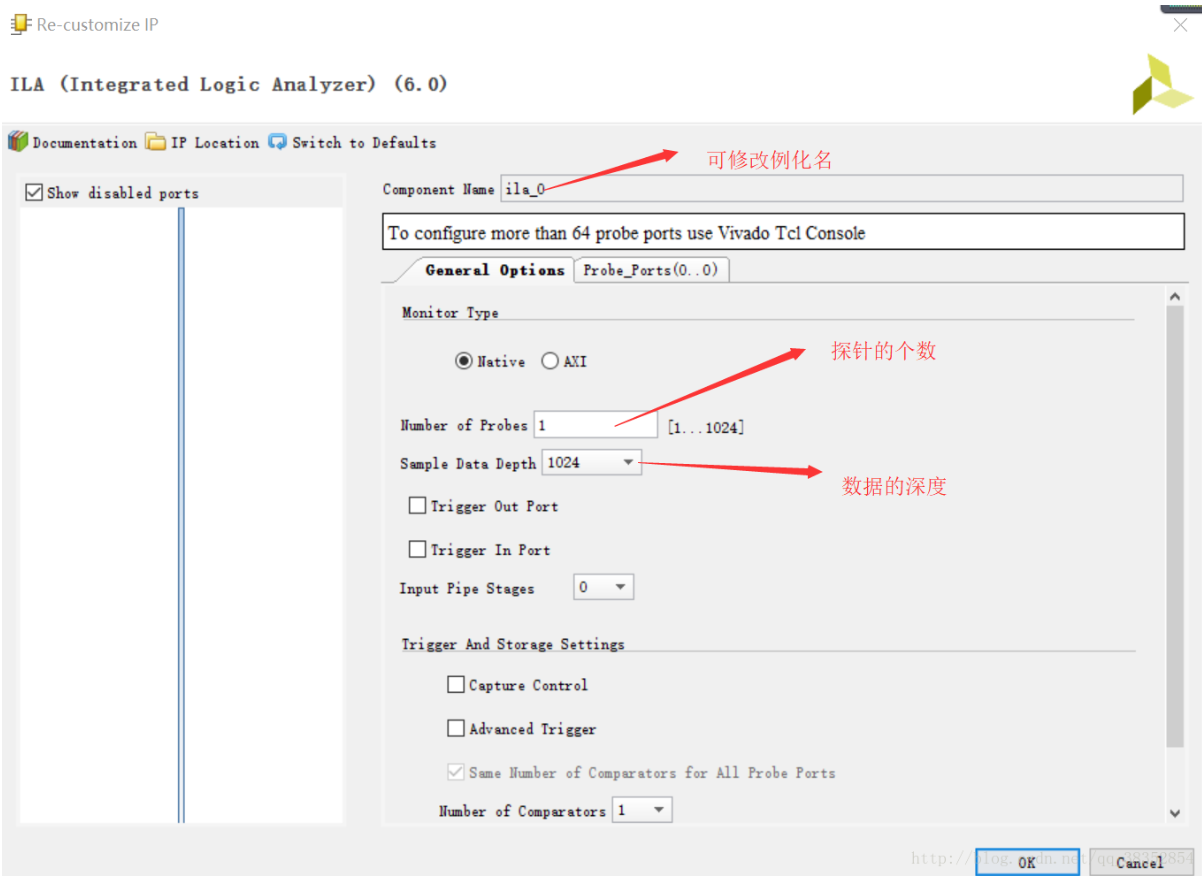
\includegraphics[width=12cm]{Figures/ILAIPConfig.png}
	\end{generalfig}

	\subsubsubsection{Vivado ILA的使用}

	综合完成后,可以打开综合界面进行“debug setup”,即配置ILA,可以在配置的时候选择采样点数、是否预触发采样、是否捕捉采样等等。一般要开启捕捉采样,方便调试。配置好ILA之后再选择实现硬件,生成比特流的操作,烧写到FPGA板子之后,便可以在运行时在线调试。
	
	
	\subsubsection{ILA调试分析}
	\subsubsubsection{ADC、采样、触发系统、FIFO、DMA综合调试}
	
	使用ILA进行调试,使用信号源对ADC输入不同频率的信号,设置不同的水平档位,处理器中控制底层数据开始采样,设置ILA触发条件为状态机跳变为预触发的状态,对模块进行综合验证调试,从而测试ADC数据、采样系统、触发系统、FIFO、DMA的功能正确性,得到以下调试图片。经过多次调试修改,验证功能正确。
	
	\begin{generalfig}[htb]{50us/div档位ILA调试图片}{fig:50usdiv}
		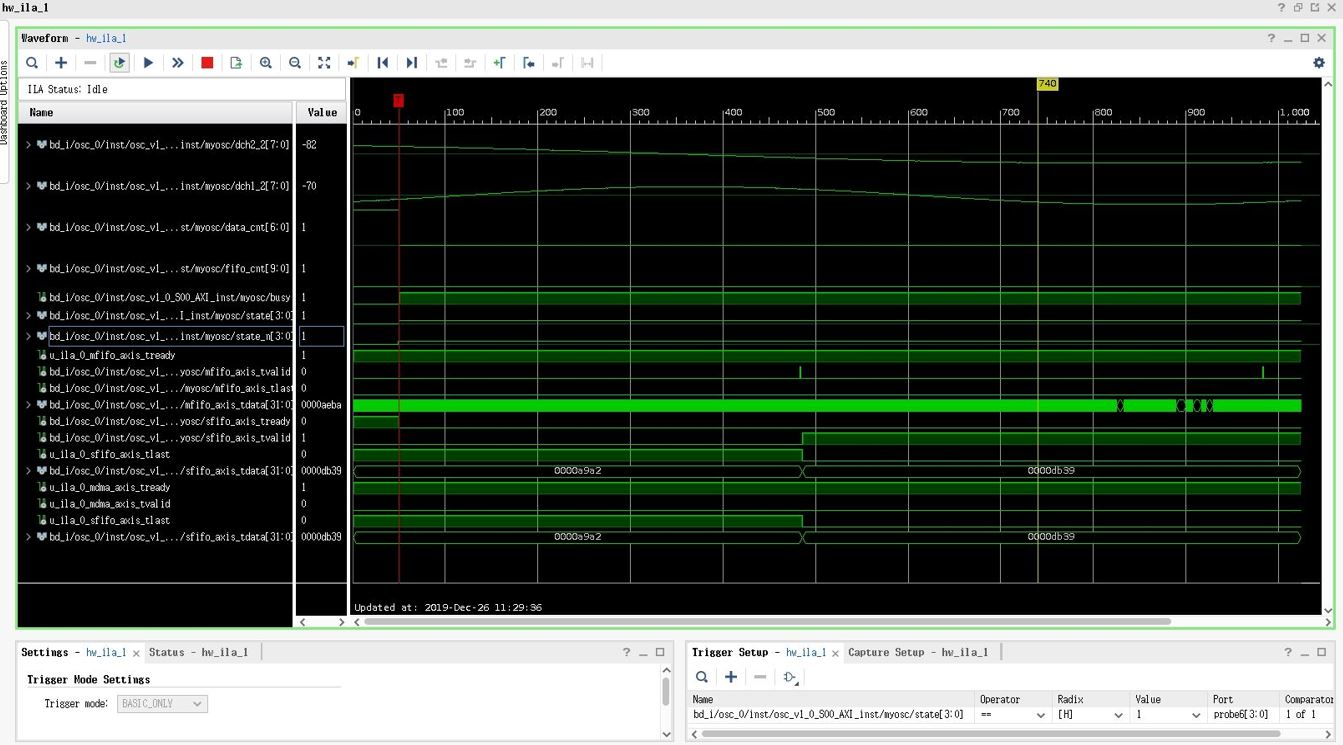
\includegraphics[width=12cm]{Figures/50usdiv.jpg}
	\end{generalfig}
	
	\begin{generalfig}[htb]{0.1us/div档位ILA调试图片}{fig:0.1usdiv}
		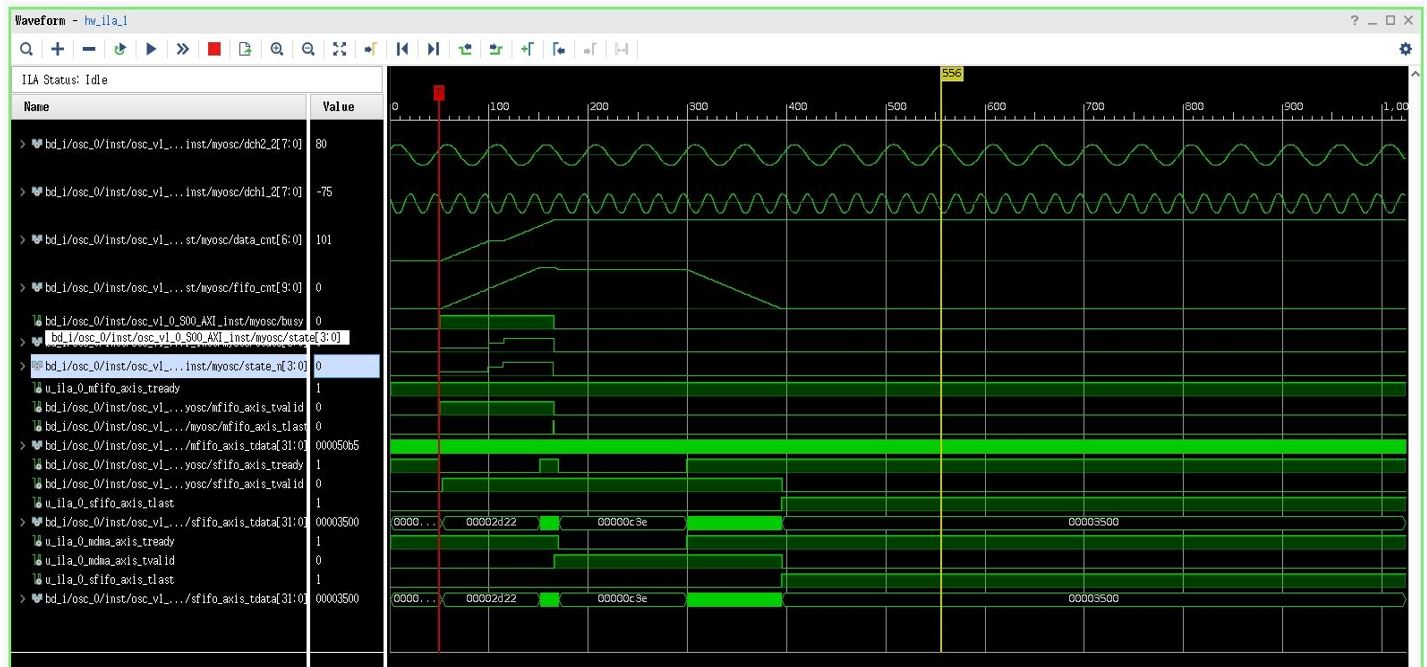
\includegraphics[width=12cm]{Figures/0.1usdiv.jpg}
	\end{generalfig}

	\subsubsection{液晶显示屏调试}

	由于液晶显示屏的时序较为清晰,故不采用嵌入式逻辑分析仪进行调试,而是直接观察输出效果。从软件顶层查看底层硬件的锁相环配置情况,即可得知显示屏的工作频率是否正确。在调试的过程中还是遇到了一些bug,有时候屏幕会进入花屏,最终发现是锁相环没有约束住,最后干脆就不采用可重构的锁相环,直接在PL部分生成一个51.2MHz的锁相环,用来给显示屏提供时钟。
	
	
	\subsubsection{人机交互界面调试}
	人机交互也是本作品的一个核心亮点,除了显示以外,还必须做触屏操作的处理,因此在触屏终端服务函数设置断点,观察每次进入这个函数(即触屏)的时候,收到的值是否正确,是否能够收到正确的值(即是否满足IIC协议)。经验证无误后再编写具体的功能服务。
	
	\subsubsection{任务调度调试}
	本设计中采用了嵌入式实时操作系统来进行任务调度,为了验证任务调度的正确性,在调试中采用了“任务中中断”的方法,对于低优先级任务,通过触屏、刷屏等高优先级任务,甚至中断,来打断它,测试优先级调度的准确性。
	
	\subsection{系统功能测试}
	在所有软件调试完成之后,我们进行了系统级的调试,主要是测试本作品的功能指标是否满足。
	
	根据题意,我们联合调试了作品的波形显示、挡位切换、触发调节、存储与调用功能、触发电平、参数测量、光标测量等功能。并用信号发生器产生各种波形来进行功能测试。最终结果也较好的反映了示波器的所有正常功能,并有部分指标超出了题目要求。如\autoref{fig:TestFigure}所示即为我们的系统功能调试照片。
	
	\begin{generalfig}[htb]{示波器整体照片}{fig:TestFigure}
		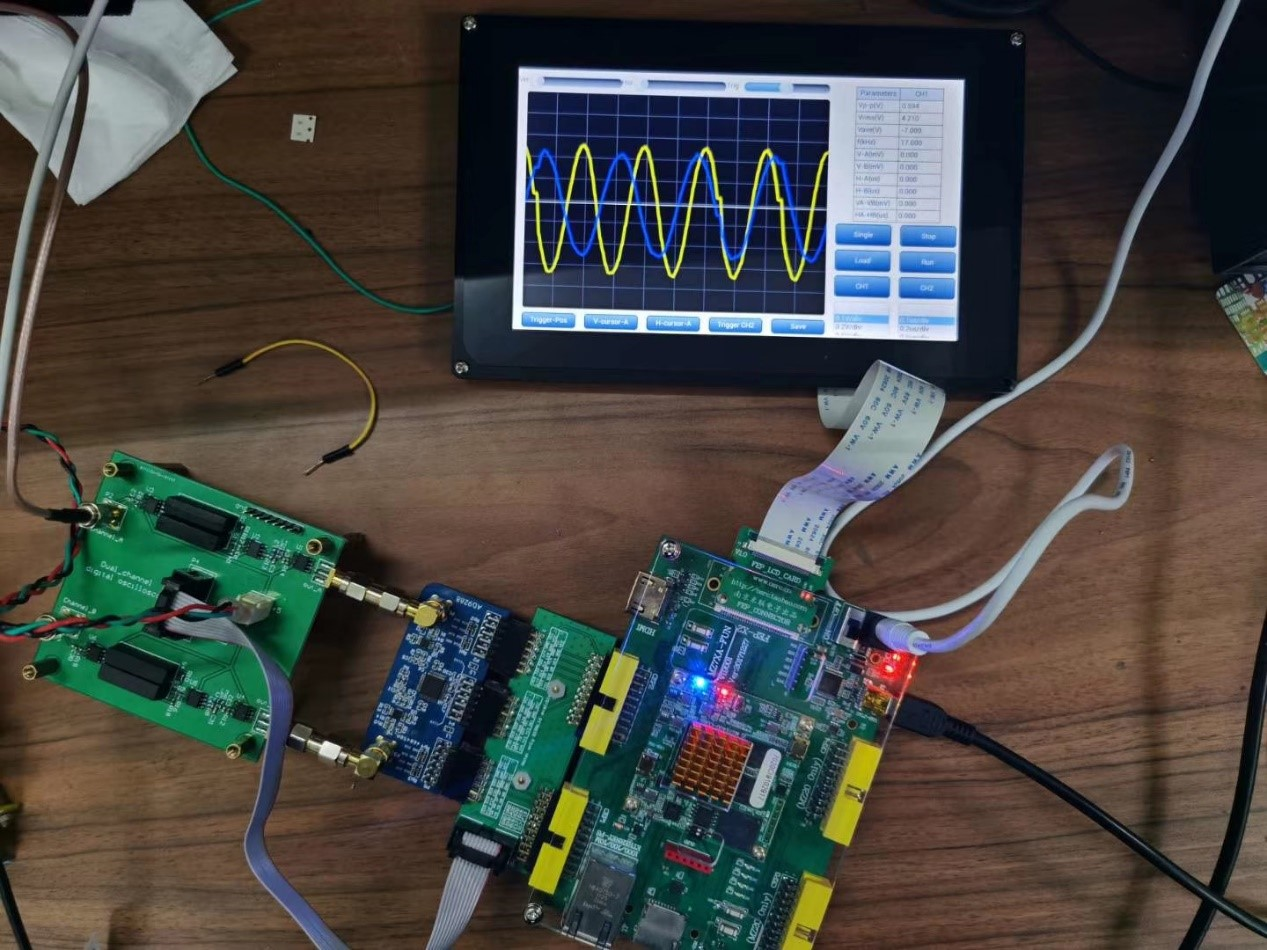
\includegraphics[width=12cm]{Figures/TestFigure.jpg}
	\end{generalfig}
	
	
	\section{测试方案与测试结果}
	
	本节单独列出系统功能测试时所采用的测试方案与系统的测试结果。
	
	\subsection{测试环境}
	\begin{generaltab}{测试环境}{tab:TestEnvironment}
		\begin{tabularx}{10cm}{lll}
			\toprule
			仪器 & 品牌 & 型号      \\
			\midrule
			示波器                   & Tektronix              & MDO2002B型数字示波器        \\
			信号发生器                 & RIGOL                  & DG1062型160M任意波形发生器    \\
			电源                    & ZhongCe                & DF1743003C型稳压源        \\
			\bottomrule
		\end{tabularx}
	\end{generaltab}
	
	\subsection{测试方案}
	
	\subsubsection{方波校准信号测试方案}
	使用示波器测试校准方波,测试其频率及幅值。
	
	\subsubsection{单次触发扫描测试方案}
	程控触发电平,观察简易数字信号示波器能否产生扫描电压,并在信号上升沿开始显示波形。
	
	
	\subsubsection{扫描速度测试方案}
	信号源输入峰峰值为1V频率可变的正弦信号,观察并记录专用示波器的周期读数,调整作品示波器各项挡位并记录数值,与标准值进
	行比较并计算误差。
	
	
	\subsubsection{垂直灵敏度测试方案}
	
	信号源输入频率为100kHz幅值可变的正弦信号,观察并记录专用示波器的幅值读数,调整作品示波器各项挡位并记录数值,与标准值
	进行比较并计算误差。

	\subsection{测试结果与数据}
	
	\subsubsection{方波校准信号测试}
	经测试,本设计产生的方波信号频率$ f=99.90\mathrm{kHz} $,峰-峰值为$ V_\mathrm{p-p}  = 0.3\mathrm{V}  $。
	
	
	\subsubsection{单次触发扫描测试}
	
	观察结果显示简易数字信号示波器能够产生扫描电压,并显示波形。如\autoref{fig:wave}所示为单次触发的显示波形。
	
	\begin{generalfig}[htb]{单次触发测试波形}{fig:wave}
		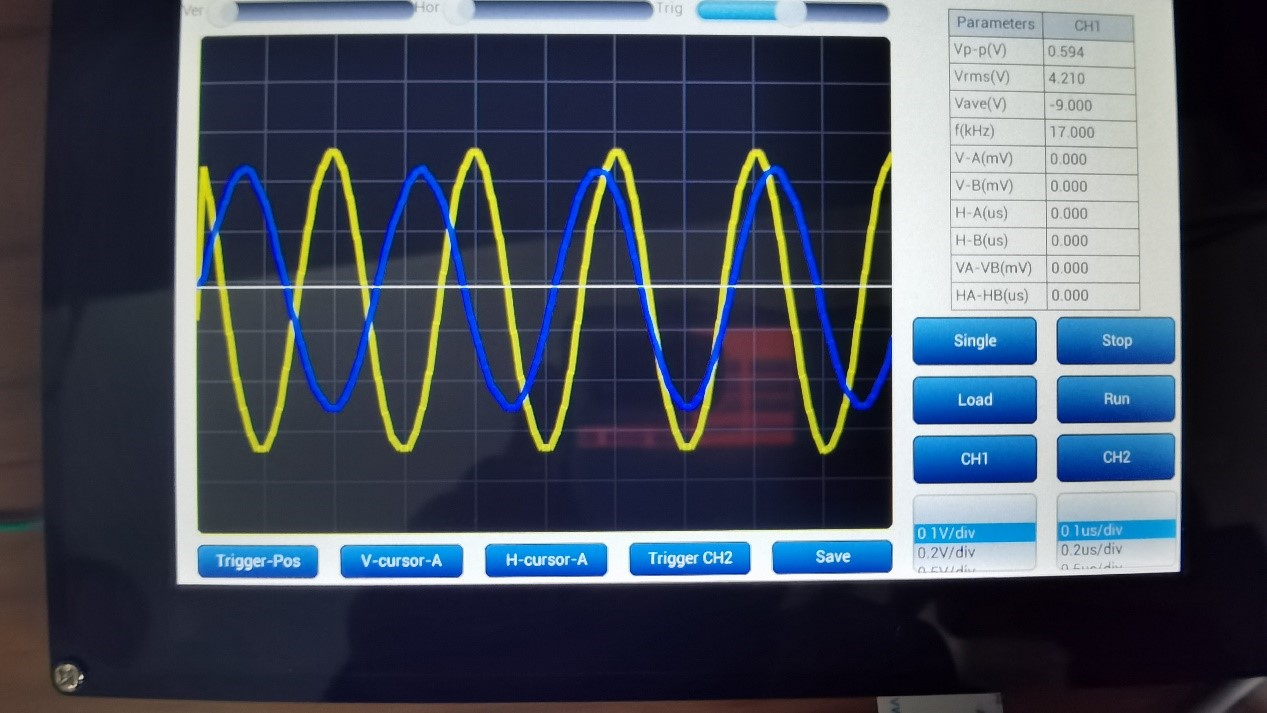
\includegraphics[width=8cm]{Figures/wave.jpg}
	\end{generalfig}
	
	
	\subsubsection{扫描速度测试}
	*信号源输入峰峰值为$ V_\mathrm{p-p}  = 1\mathrm{V}  $的正弦信号。

	\begin{generaltab}{扫描速度(周期)测试表}{tab:PeriodTest}
		\begin{tabularx}{10cm}{CCCC}
			\toprule
			\multirow{2}{*}{扫描速度} & \multicolumn{3}{c}{周期} \\ \cmidrule(l){2-4} 
			& 实际值    & 测量值    & 误差   \\ 
			\midrule
			\multirow{3}{*}{10us/div}  & 50us   & 49.0us & 2.0\% \\
			& 20us   & 20.4us & 2.0\% \\
			& 10us   & 10.0us & 0     \\ 
			\midrule
			\multirow{3}{*}{1us/div}   & 5us    & 5.2us  & 4.0\% \\
			& 2us    & 2.02us & 1.0\% \\
			& 1us    & 1.04us & 4.0\% \\
			\midrule
			\multirow{3}{*}{100ns/div} & 1000ns & 982ns  & 1.8\% \\
			& 500ns  & 516ns  & 3.2\% \\
			& 100ns  & 96ns   & 4.0\% \\ 
			\bottomrule
		\end{tabularx}
	\end{generaltab}

	\subsubsection{垂直灵敏度测试}
	*信号源输入频率为$ f = 100\mathrm{kHz} $的正弦信号。
	\begin{generaltab}{垂直灵敏度测试表}{tab:HTest}
		\begin{tabularx}{10cm}{CCCC}
			\toprule
			\multirow{2}{*}{垂直灵敏度}    & \multicolumn{3}{c}{幅值} \\ \cmidrule(l){2-4} 
			& 实际值    & 测试值   & 误差    \\ \midrule
			\multirow{3}{*}{0.5V/div} & 1V     & 1.01  & 1\%   \\
			& 2V     & 2.02V & 1\%   \\
			& 4V     & 4.07V & 1.7\% \\ \midrule
			\multirow{3}{*}{0.2V/div} & 400mV  & 412mV & 3.0\% \\
			& 800mV  & 787mV & 1.6\% \\
			& 1.6V   & 1.62V & 1.3\% \\ \midrule
			\multirow{3}{*}{0.1V/div} & 200mV  & 204mV & 2.0\% \\
			& 400mV  & 410mV & 2.5\% \\
			& 800mV  & 822mV & 2.7\% \\ \bottomrule
		\end{tabularx}
	\end{generaltab}


	\subsection{测试结果分析}
	
	根据题意,联合调试了作品的波形显示、挡位切换、触发调节、存储与调用功能、触发电平、参数测量、光标测量等功能。并用信号发生器产生各种波形来进行功能测试。最终结果也较好的反映了示波器的所有正常功能,并有部分指标超出了题目要求。
	
	
	\section{问题分析与总结}
	\subsection{问题分析}
	\subsubsection{数字示波器硬件问题}
	在数字示波器这个课设作品中,刘刚负责的主要是前端信号调理电路和AD采样电路这两个模块,整个设计的过程比较简单,需要注意的地方是信号调理电路中运放的选型,既要保证足够的带宽,使能处理的信号频带尽可能大,又要尽可能挑选单位增益稳定的精密运放。最开始刘刚选用了TI公司的精密运放OPA820构成第一级的跟随器,但是效果并不好,跟随后的信号波形出现了严重失真,最后经过换过几次运放后,选择了OPA656,它的输入失调参数都较小,能够很好的实现有关功能。
	
	
	\subsubsection{数字示波器软件问题}
	课设的过程中,我们第一次尝试写数字示波器的代码,过程中我们遇到了很多问题,在此罗列一些在过程中遇到的问题。
	
	1、在多个过程块中对同一变量赋值
	
	开始我们按照自己的思路,将各个功能模块用verilog写了出来,但是刚开始我们的思维还没有完全从C语言、汇编这类框架中跳脱出来,也没有完全领悟到verilog“硬件描述语言”的本质,它描述的是电路状态,最终也要被映射成实际电路,我在不同的过程块中对同一变量进行赋值,实际就相当于电路中的“线与”,这种情况是应该被避免的,而我们等到modelsim仿真编译时出现很多error才发现这个问题,然后又是重新捋清思路,一点点改代码,直到没有error。
	
	2、按键消抖的边沿触发问题
	
	按键消抖模块的原理是每隔50ms分别读取按键的电平,然后对读出的值做异或运算。一般来说,一次合法的按键按下,会产生两个脉冲,将两个波形分别存储,分别过D触发器然后就会得到一个表示按键被按下的脉冲,持续时间为一个周期,然后可以用电平检测的方法来判断按键是否被按下。在写这段代码的过程中,按键按下的时候变为低电平,所以应该判断下降沿来决定是否产生第一个脉冲,然后过D触发器合成一个脉冲,结果分析modelsim波形图的时候却发现最后的指示脉冲出现在了测试代码里按键松开后,相当于多了一段延时,我们向同学请教才发现是最后产生脉冲时非逻辑的对象给错了,然后才改了过来。
	
	3、其它一些问题
	
	这次写整体的verilog代码,我们也犯了很多粗心的错误,比如阻塞性赋值与非阻塞性赋值出现在同一个过程块里、使用的端口未声明、编写测试代码是变量类型定义错误等等。出现这些问题主要还是因为经验不足,写代码不够熟练,我相信多经过几次练习,这种错误出现几率一定会大大降低。
	
	
	\subsection{心得感悟}
	这次电子课程设计我们完成的双通道数字示波器能够满足题目中的要求,而且采样率达到100M,输入信号的范围也可达5M,应该算是一个不错的作品。
	
	整个过程中我最大的感悟:要学会FPGA,一定要实践实践多实践,只有真正尝试去做了,才会明白过程中有多少坑,然后一点一点把不会的地方学会,把存在的问题解决,逐渐积累经验,最后完成一个作品时才能游刃有余。
	
	
	
	
	\section{参考文献}\label{sec:ref}
	
	[1].	罗杰.Verilog HDL与数字ASIC设计基础,2008,华中科技大学出版社.
	
	[2].	王贞炎.FPGA应用开发和仿真,2018,机械工业出版社.
	
	[3].	[美]Bruce Carter.运算放大器权威指南(第四版),2014,人民邮电出版社.
	
	[4].	谭浩强.C语言程序设计,2010,清华大学出版社.
	
	[5].	陈尚松.电子测量与仪器(第四版),2018,电子工业出版社.
	
	%生成参考文献
	%使用方法:\bibliography{参考文件1文件名, 参考文献2文件名, ...}
	%\bibliography{Bibs/mybib}
	
	\begin{appendices}
		\section{【2007国赛C题】数字示波器}
		
		
		
		\begin{generalfig}[htb]{数字示波器-1}{fig:Question1}
			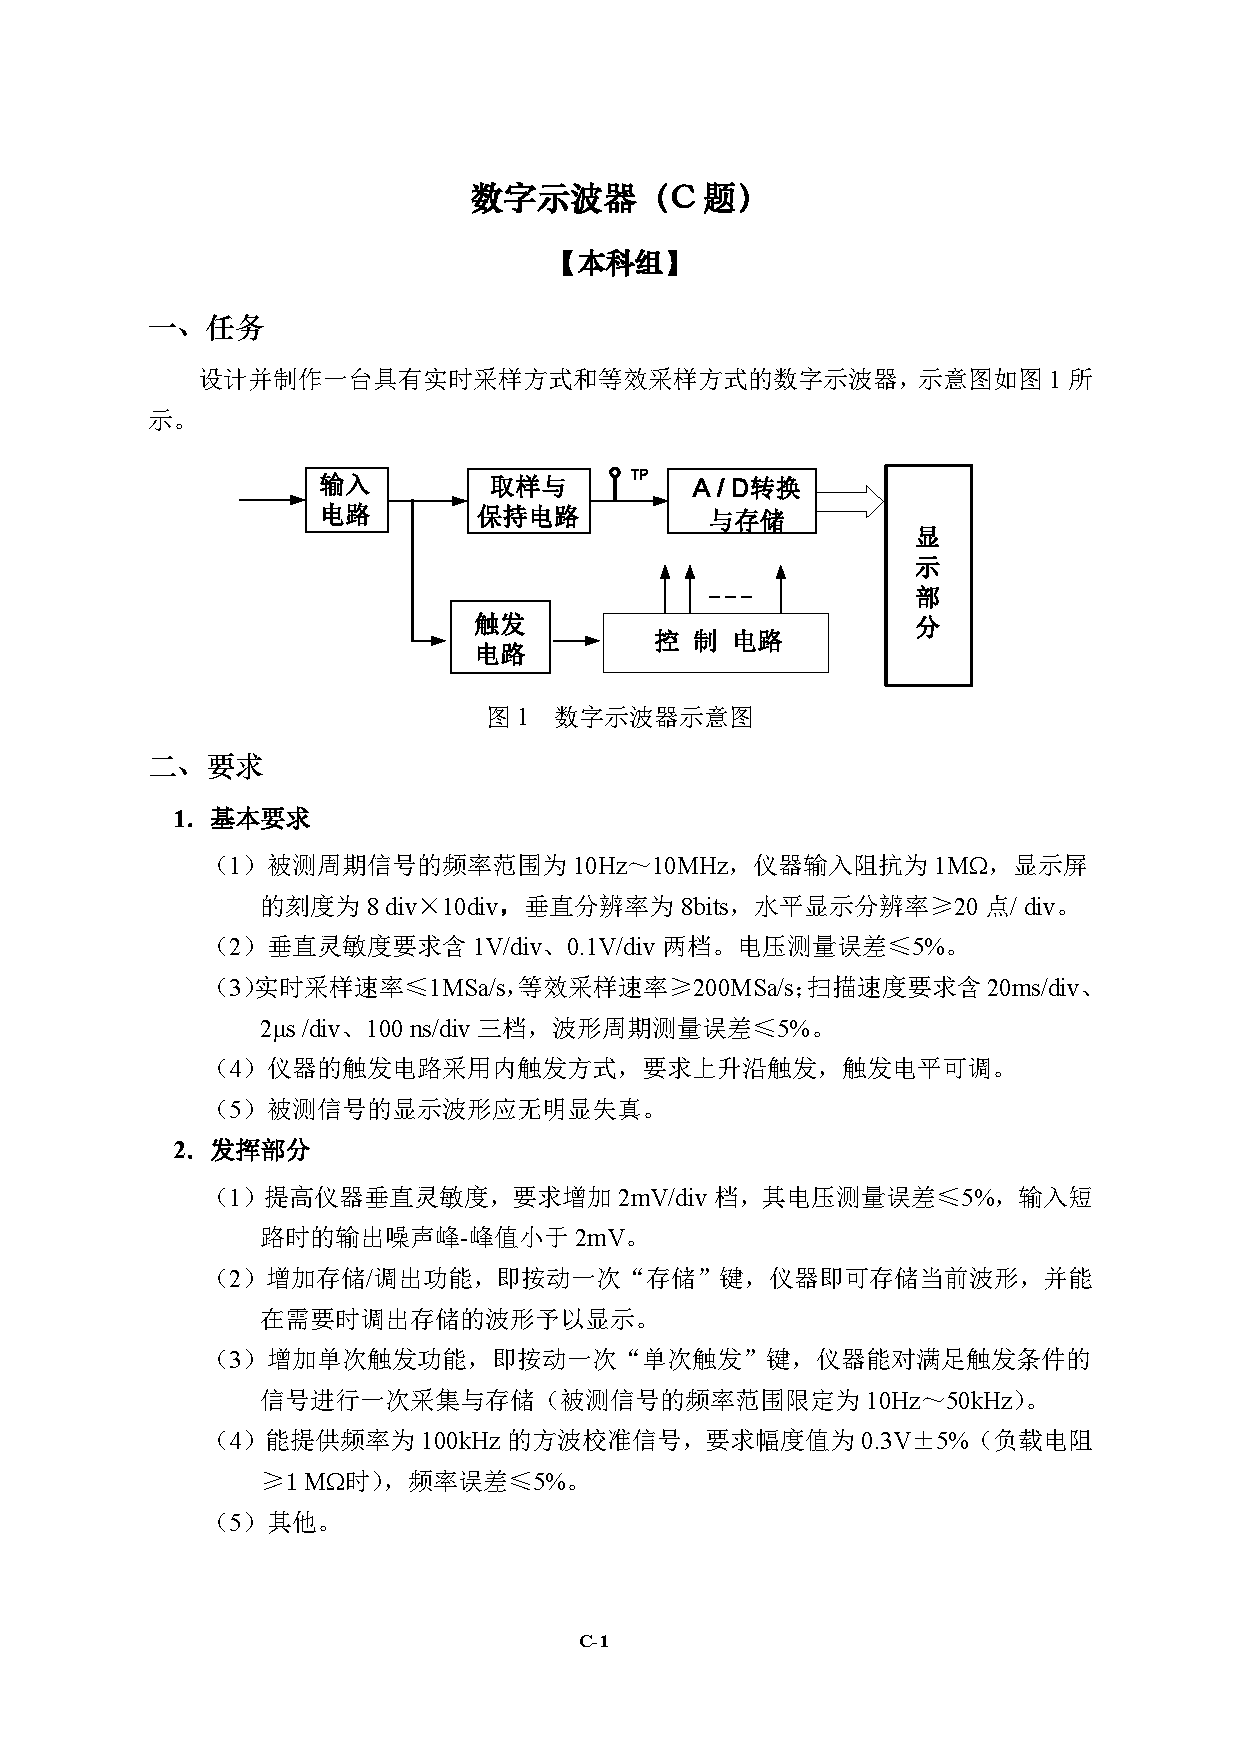
\includegraphics[width=13cm,page=1]{Docs/Question.pdf}
		\end{generalfig}
	
		\begin{generalfig}[htb]{数字示波器-2}{fig:Question2}
			\includegraphics[width=13cm,page=2]{Docs/Question.pdf}
		\end{generalfig}
	
		\section{平台说明及主要元器件清单}
		本设计使用的FPGA开发平台为米联客MZ7XA XILINX FPGA开发板,MZ7XA是米联电子Zynq-7000系列开发平台一款全新的高端产品。其性价比高、资源丰富,拥有摄像头、HDMI、千兆以太网、FEP等众多高性能接口,适合用于本设计的开发。FPGA开发平台如\autoref{fig:FPGABoard}所示。
		
		\begin{generalfig}[htb]{FPGA开发平台}{fig:FPGABoard}
			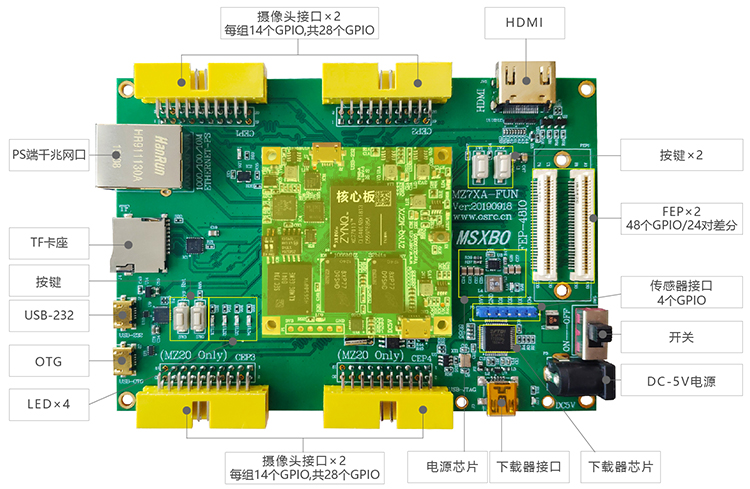
\includegraphics[width=12cm]{Figures/FPGABoard.jpg}
		\end{generalfig}
	
		平台及主要元器件清单如\autoref{tab:BOM}所示。
		\begin{generaltab}{平台及主要元器件清单}{tab:BOM}
			\begin{tabularx}{10cm}{CC}
				\toprule
				元件种类& 元件型号       \\
				\midrule
				开发平台 & 米联客MZ7XA      \\
				模数转换器 & AD9288     \\
				运算放大器 & OPA656     \\
				运算放大器 & OPA820     \\
				高速差分放大器 & AD8132     \\
				\bottomrule
			\end{tabularx}
		\end{generaltab}
	
	\end{appendices}
	
\end{document}
